\section{Proposed Work}\label{section-proposed-work}
In general to generate BIOS image (*.rom file), compilation of XYZ.c (source code) has to be done, this compilation not only involves compilation of DXE driver, PEI driver, EFI Application but also includes pre-processing checks, compression of raw files which takes huge amount of time depending on the system configuration. Implementation of this project aids in reduction of this compilation time.

\subsection{Stack holders}\label{subsection-stack-holders}
The proposed work is applicable but not limited to below stack holders:
\begin{itemize}
	\item \textbf{BIOS development team} : main development group in contributing BIOS firmware, this is the only stockholder who are having access to the BIOS development environment and access to the source code of the complete BIOS firmware
	\item \textbf{Validation team} : performs various validation on developed BIOS image
	\item \textbf{Automation team} : brings various integration and validation automation to module(s)
	\item Other Development team who wishes to ease the debugging process
\end{itemize}

\subsection{Issues}\label{subsection-issues}
The Proposed work is capable of mitigating below issues:
\begin{itemize}
	\item Generation of BIOS image - includes compilation of whole source code
	\item Time complexity - took enormous amount of time to generate the BIOS image
	\item Accessing and modifying BIOS Setup Option(s) remotely
	\item Firmware Flashing of BIOS remotely
	\item Updating CPU microcode
	\item Summarizing changes among BIOS image
	\item Avoiding exposing the source code support for OEM to fill their OEM information
	\item Avoid setting of BIOS development platform for stack holders which are not meant to be the BIOS developer
	\item Runtime BIOS Support for temporary UEFI variable creation
\end{itemize}

\subsection{Requirements}\label{subsection-requirements}
\subsubsection{Software Requirements}
\begin{itemize}
	\item Visual C/C++ binaries
	\item Python 3
	\item Visual Studio Code (IDE)
	\item Memory Access Interface - supported mechanism to communicate over target memory
\end{itemize}

\subsection{Development Process of Modules}
Framework development process is driven by implementation of independent modules which can serve functionality and having flexibility to integration to the framework.


% ========================================================================
% MODULE 1
% ========================================================================

%\subsection{Module 1: Processing Firmware individually}\label{subsection-processing-firmware}
%To process apply the whole firmware changes individually for BIOS, signing is require to be performed for individual Firmware before stitching it to the BIOS binary in the valid structure.
%
%\subsubsection{Primary Goals of the module}
%\begin{itemize}
%	\item Remove other Intellectual Property's dependency (\gls{ip} dependency) during firmware loading
%	\item \gls{ip} Subsystem :
%	\begin{itemize}
%		\item Loader and Verifier
%		\item \gls{ip} is always consumer
%	\end{itemize}
%	\item Signature verification using \gls{sha} hash algorithm and should be ease support for adding new algorithmic support as needed.
%	\item Should support hardware based and software based verification support
%	modifying memory requirements for given IP without impacting eco-system
%	\item Prevent common security threats
%	\item Allow easier OEM adoption and modification based on the respective design
%	\item Reusability/Portability of design across many \gls{ip}s
%	\item Generic design which supports any new IP integration
%\end{itemize}
%
%\begin{figure}[!htbp]
%	\centering
%	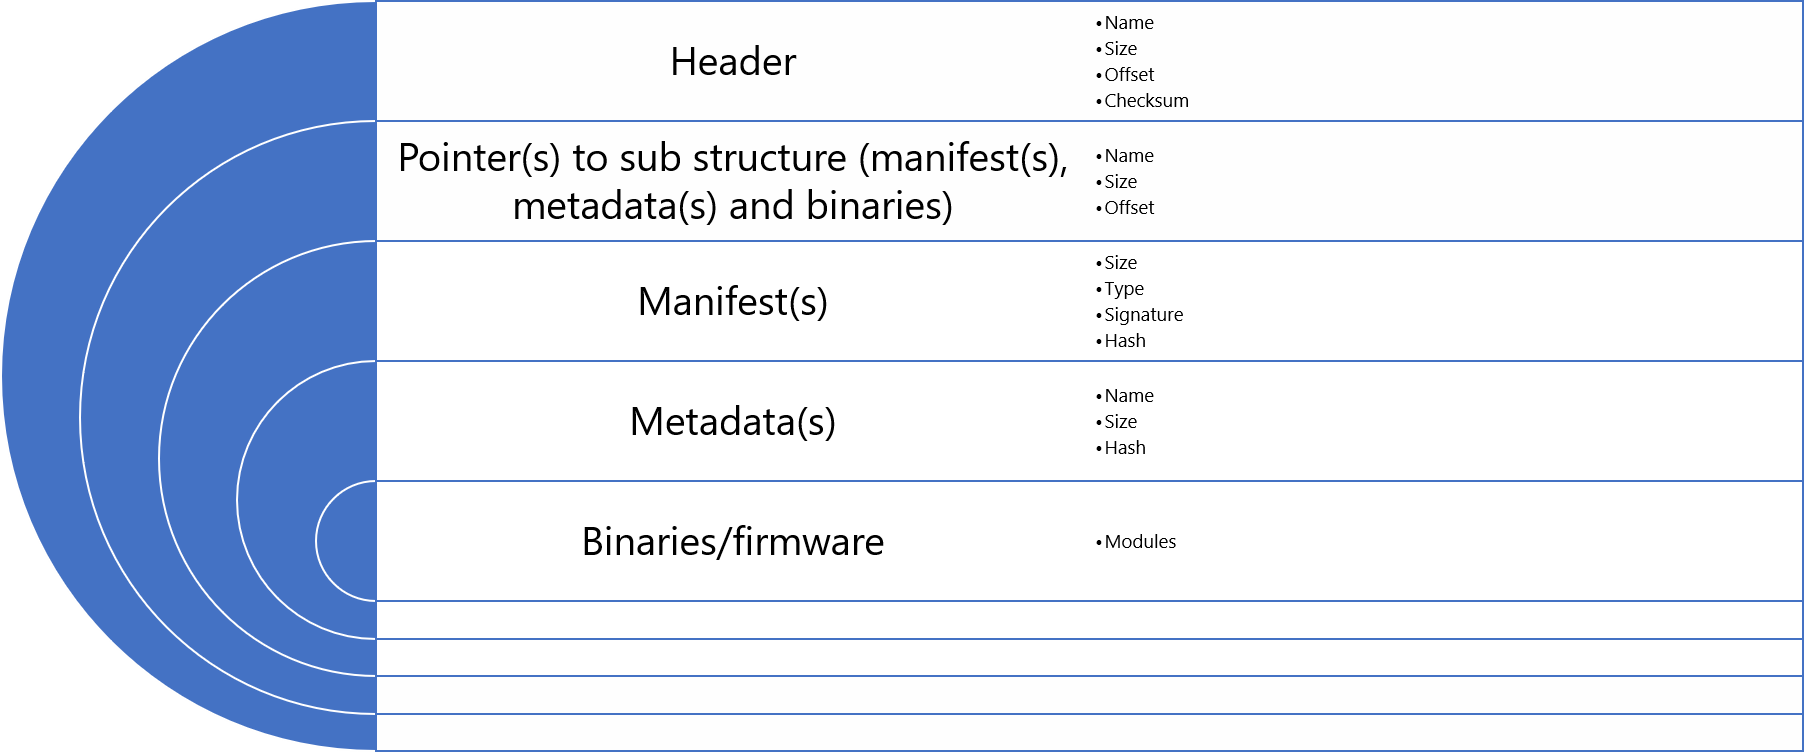
\includegraphics[width=\linewidth]{proposed-work/proposed-structure-firmware-signing}
%	\caption{Proposed Structure for firmware signing}\label{fig:proposed-work-proposed-structure-firmware-signing}
%\end{figure}
%
%Note: Due to Confidentiality other details of this module is not to be disclosed such as flow diagram, structures or pseudo code.

% ========================================================================
% MODULE 1
% ========================================================================
\subsection{Module: Setup Knob modification}\label{module-setup-knob-modification}

\subsubsection{Processing Unsigned debug BIOS}\label{subsection-processing-bios}
Before Releasing the BIOS firmware for public use, those are signed for security and integrity purpose, however the debug BIOS which are used Pre-release to test and verify all the functional features until all the requirements are met.

Every \gls{soc} system which are under test known is \gls{sut} are configured in such a way that it supports debug BIOS. The proposed framework is designed to simulate the process of \gls{sut} in terms of processing BIOS binary similar to \gls{sut} performs it after flashing BIOS firmware on \gls{soc}.

Processing the debug BIOS can be classified in to two ways:
\begin{enumerate}\label{cli-classification-proposed-work}
	\item Applying changes directly to the \gls{sut}
	\item Applying changes on to the BIOS image
\end{enumerate}

At the high level the flow for both the above classification remains the same but will be differentiated at the backend support. An additional driver is attached with BIOS firmware to aid the framework to be able to apply changes directly to the \gls{sut}.

\subsubsection{Additional Tech Stack Used}
Below are the listed technologies consumed in development of this module in addition to the already specified requirements in Section \ref{subsection-requirements}
\begin{itemize}
	\item Tkinter
	\item XML
	\item JSON
\end{itemize}

\subsubsection{Flow of the module}
Figure \ref{fig:setup-knobs-flow} describes the flow of setup knobs modification on the System Under Test (SUT).

\begin{figure}[!htbp]
	\centering
	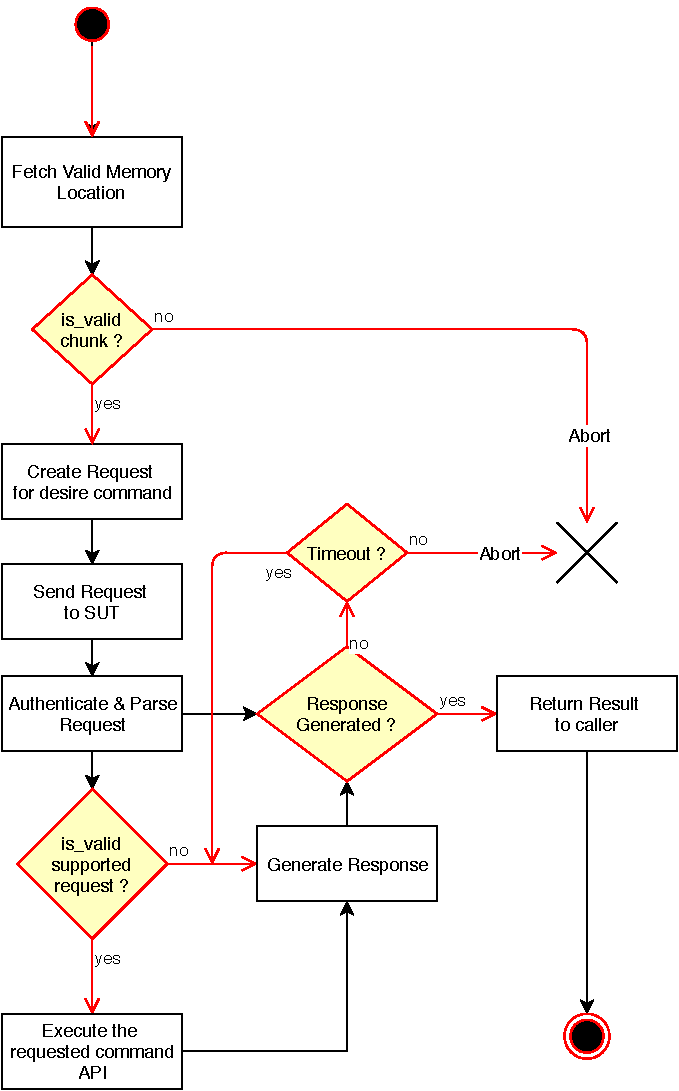
\includegraphics[width=0.9\linewidth]{proposed-work/setup-knobs-flow}
	\caption{Flow of Setup Knobs Modification}\label{fig:setup-knobs-flow}
\end{figure}

The iteration of the development could be reduce in two ways:
\begin{enumerate}
	\item Processing Debug/Unsigned BIOS in section \ref{subsection-processing-bios}
	\item Processing Firmware individually in section \ref{subsection-processing-firmware}
\end{enumerate}


\subsubsection{Screenshots of Module}
As a \gls{poc} for the framework, this section shows snapshots of the working module to mimic the setup options of BIOS, however as a simulation framework, it also provides quite more features which are not available in the actual BIOS due to memory limitation.

Figure \ref{fig:proposed-work-bios-gui-initial-config} shows the prompt asked to user to select basic configurations before launching the module of framework. Configurations available to select are:

\begin{itemize}
	\item Working Mode (options to be selected as in figure \ref{fig:proposed-work-bios-gui-initial-config-select-mode})
	\begin{itemize}
		\item \verb|online| - to work on \gls{sut} and require to select valid access method for online mode from menu
		\item \verb|offline| - to work on BIOS binary
	\end{itemize}
	\item Access Method - selecting valid access method for working on \gls{sut}
	\item Publish all? - Boolean options to decide whether to evaluate \gls{depex} or not.
\end{itemize}

\begin{figure}[!htbp]
	\centering
	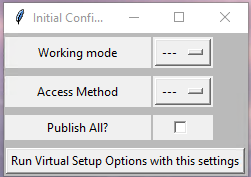
\includegraphics[width=0.7\linewidth]{proposed-work/bios-gui-initial-config}
	\caption{Menu to Select initial configuration for work}\label{fig:proposed-work-bios-gui-initial-config}
\end{figure}

\begin{figure}[!htbp]
	\centering
	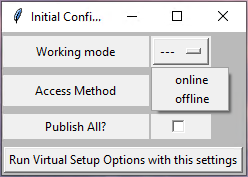
\includegraphics[width=0.7\linewidth]{proposed-work/bios-gui-initial-config-select-mode}
	\caption{Available work mode for the system: Online and Offline}\label{fig:proposed-work-bios-gui-initial-config-select-mode}
\end{figure}


%Figure \ref{fig:proposed-work-bios-gui-acpi-knobs} shows the view that how an options in the module simulation is loaded.

\begin{table}
	\centering
	\renewcommand{\arraystretch}{2}
	\caption{Interpretation of buttons on Virtual Setup Page GUI}\label{table:interpretation-of-buttons-in-module}
	\begin{tabular}{l | p {8cm}}
		Button & Interpretation
		\\ \hline \hline
		Push Changes & Apply changes to system if online mode else apply changes to `bin` file
		\\ \hline View Changes & View saved changes in new window
		\\ \hline Exit & Exit the GUI
		\\ \hline Reload & Reload the GUI
		\\ \hline Discard Changes & Discard any change made, any value if modified are restored to current value
		\\ \hline Load Defaults & Restore to default values and revert any changes made
		\\ \hline
	\end{tabular}
\end{table}

%\begin{figure}[!htbp]
%	\centering
%	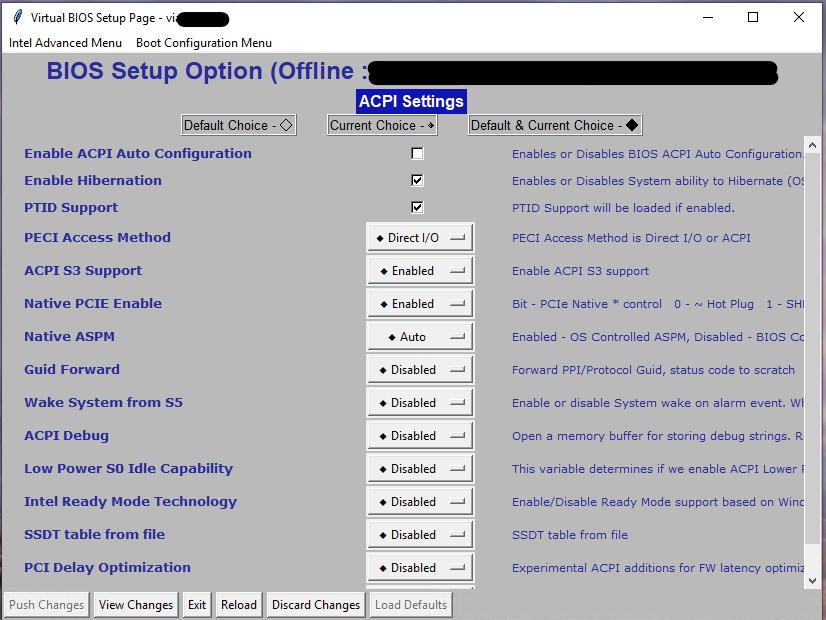
\includegraphics[width=0.8\linewidth]{proposed-work/bios-gui-acpi-knobs}
%	\caption{Setup Options listed under ACPI Configurations}\label{fig:proposed-work-bios-gui-acpi-knobs}
%\end{figure}

Table \ref{table:interpretation-of-buttons-in-module} describes the interpretation of each button action on specific condition as remarks if applicable


%Navigation through the various BIOS pages can be done as shown in Figure \ref{fig:proposed-work-bios-gui-accessing-menu}.

%\begin{figure}[!htbp]
%	\centering
%	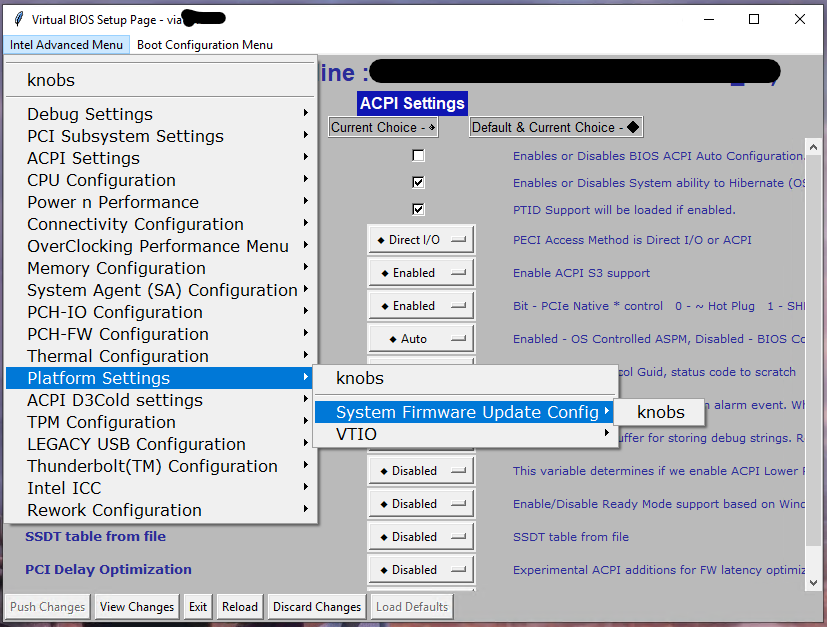
\includegraphics[width=0.8\linewidth]{proposed-work/bios-gui-accessing-menu}
%	\caption{Navigating through BIOS setup page}\label{fig:proposed-work-bios-gui-accessing-menu}
%\end{figure}

%Figure \ref{fig:proposed-work-bios-gui-view-changes} displays list of changes made in setup options across any setup page and listed separately to compare with previous value, discard or apply the new values.

%\begin{figure}[!htbp]
%	\centering
%	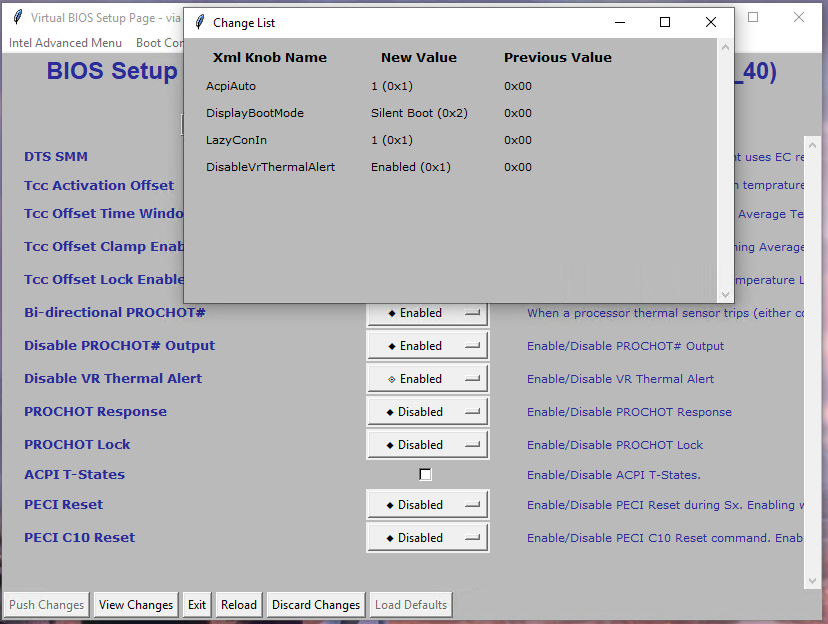
\includegraphics[width=\linewidth]{proposed-work/bios-gui-view-changes}
%	\caption{Viewing all the changes made during current session}\label{fig:proposed-work-bios-gui-view-changes}
%\end{figure}

\subsubsection{Outcome of Module}
\begin{itemize}
	\item The module is capable of cross platform usage.
	\item The module can work with all the platform binary and \gls{sut}.
	\item A communication bridge as a driver in BIOS firmware to aid the framework run directly on \gls{sut} is implemented.
	\item Generic solution is provided for end-user while running any of the classification listed in \ref{cli-classification-proposed-work}.
	\item Simulating the information from system or binary image is provided as native GUI application.
	\item Real time sync with simulation framework is supported.
	\item Seamless Integration of any new features or modules in framework is made possible.
\end{itemize}

% ========================================================================
% MODULE 2
% ========================================================================
\subsection{Module: Parsing}\label{module-parsing}
Figure \ref{fig:bios-as-filesystem} represents the overview of the BIOS as a File system  which is interpreted and parsed from the BIOS image. Detail architecture of the same is explained in Section \ref{section-architecture}

\begin{figure}[!htbp]
	\centering
	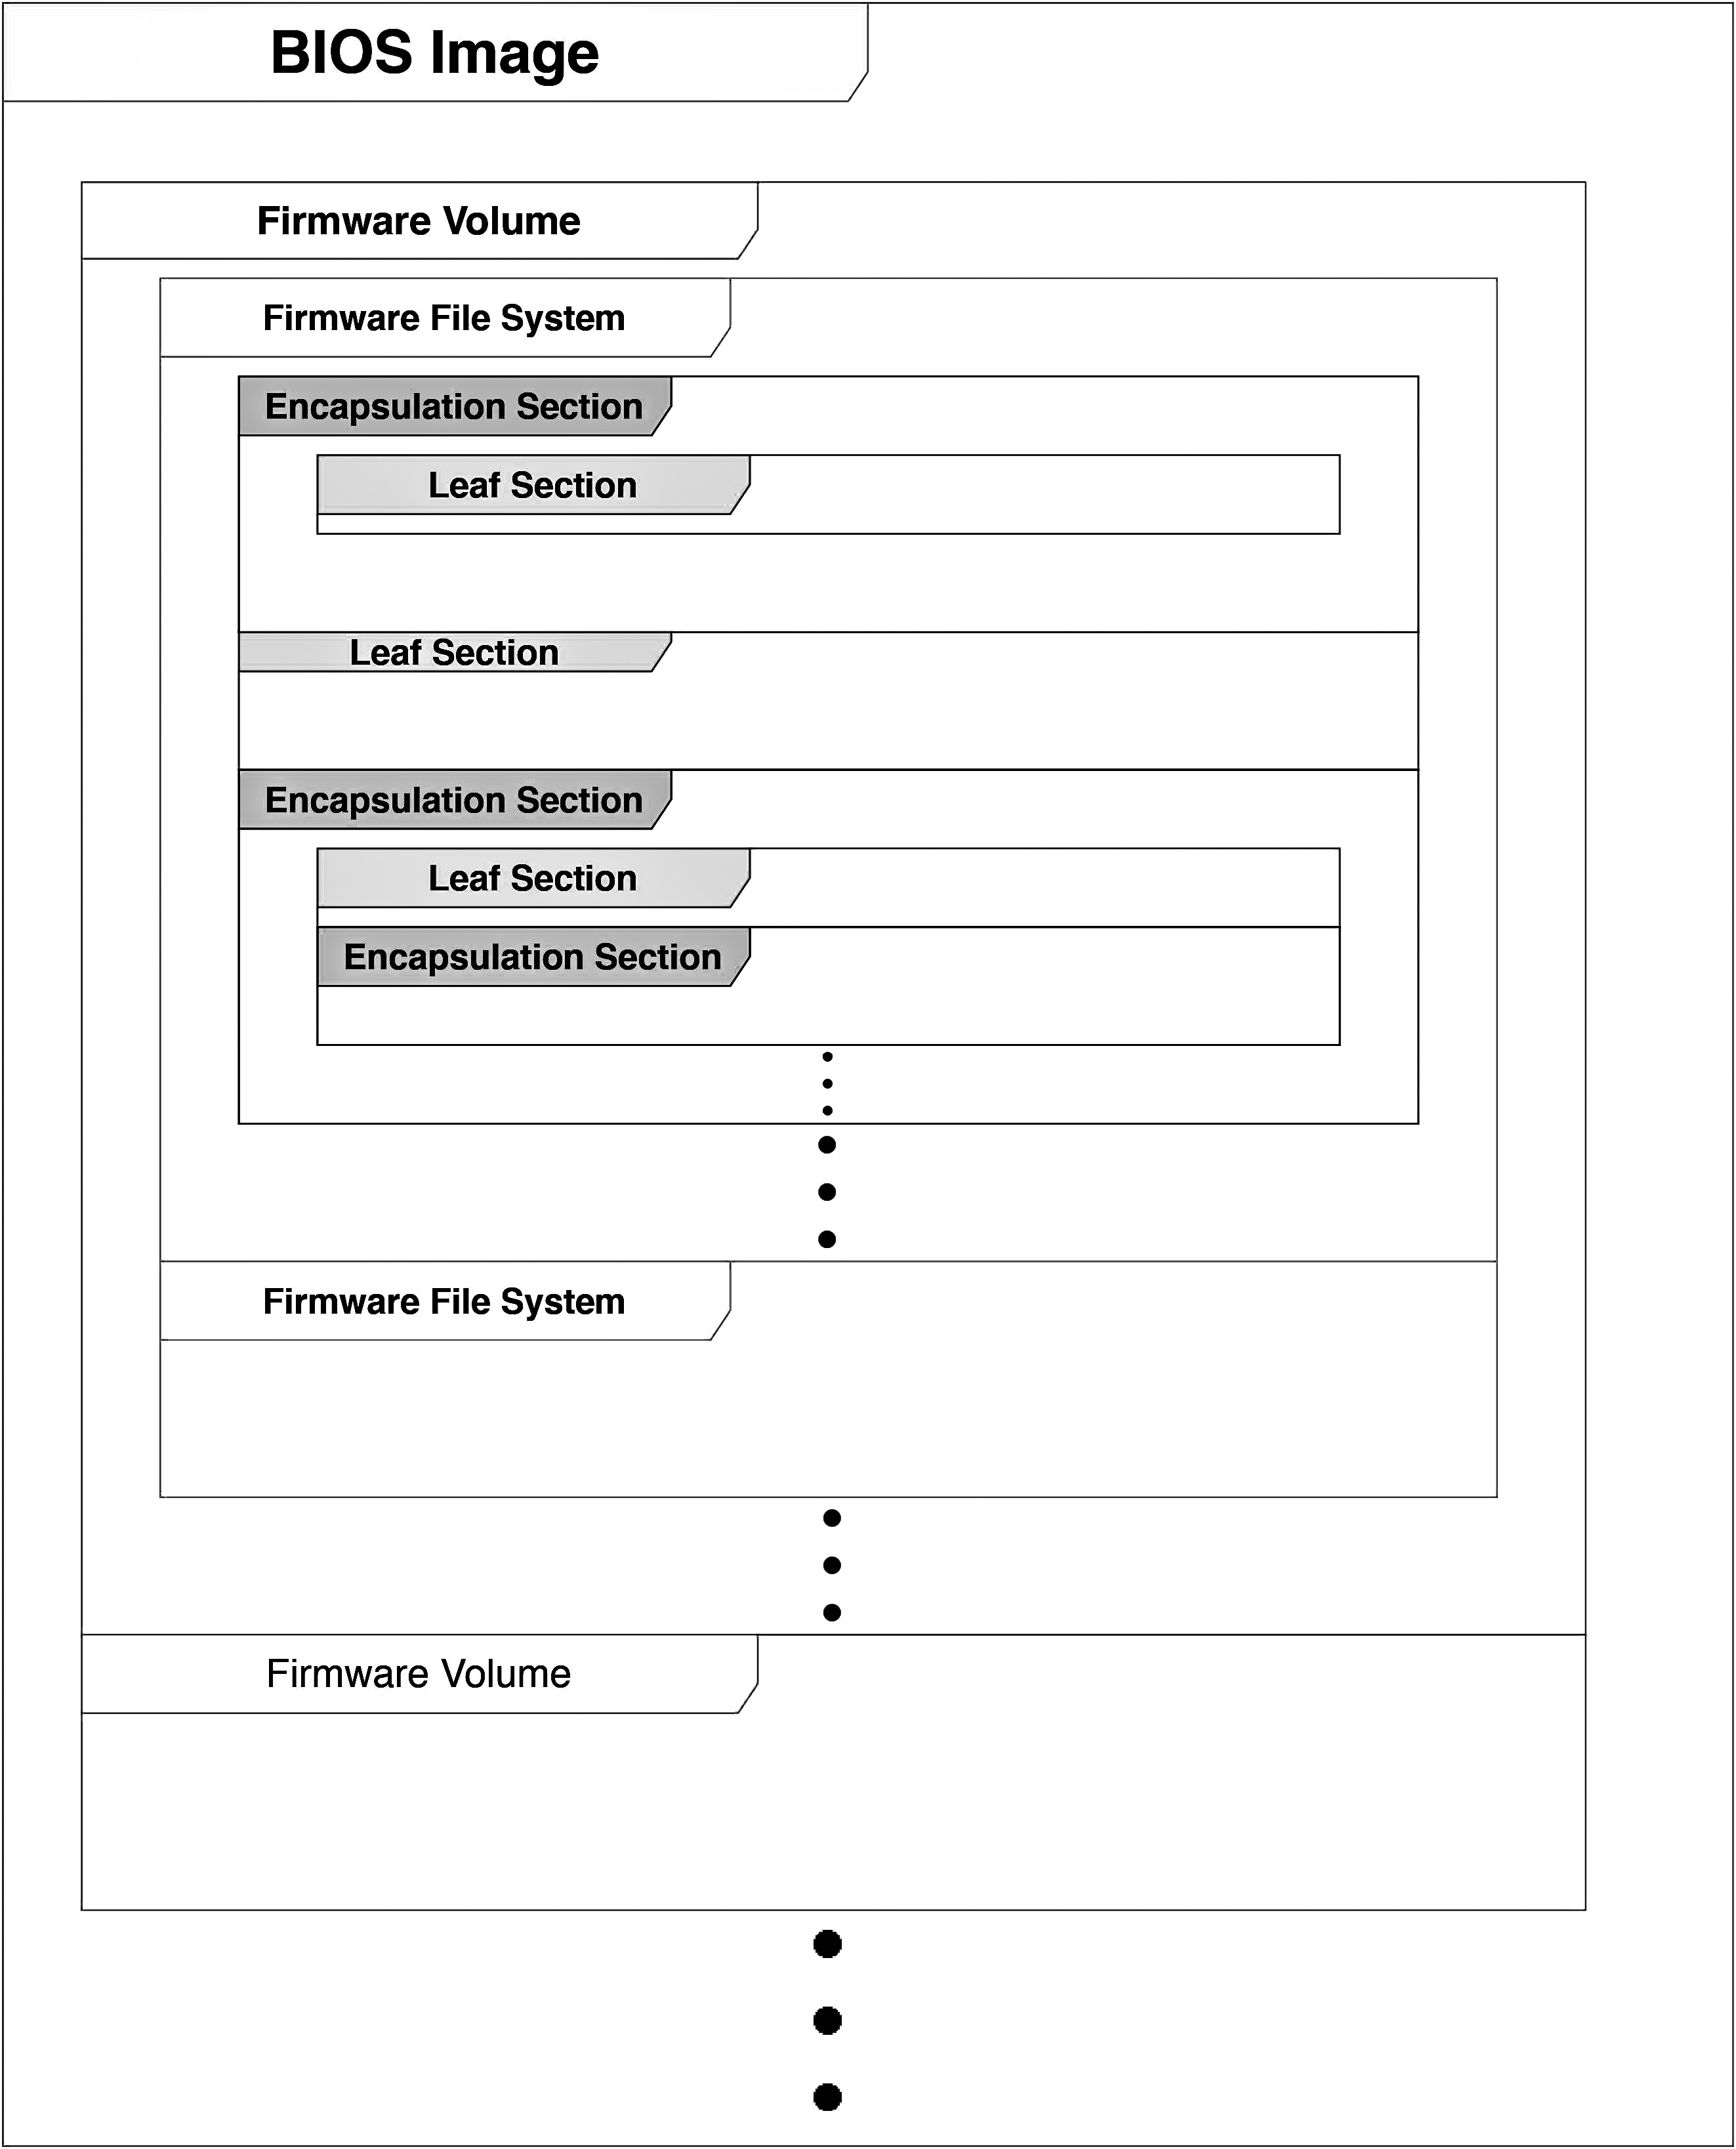
\includegraphics[width=\linewidth]{proposed-work/bios-as-filesystem}
	\caption{Overview of BIOS image as a File System}\label{fig:bios-as-filesystem}
\end{figure}

\subsubsection{Additional Tech Stack Used}
Below are the listed technologies consumed in development of this module in addition to the already specified requirements in Section \ref{subsection-requirements}
\begin{itemize}
	\item Decompression binaries
	\item XML
	\item JSON
\end{itemize}

\subsubsection{Flow of the module}
Figure \ref{fig:uefi-parser} describes the flow of the Parsing module. The Initial part is performed by user who is responsible to select valid memory interface to work. Note that some memory interface are supported by the module which requires additional hardware and software setup which are considered to be the part of dependency of interface itself which is not in the scope of the module.

When User select valid Interface the module will determine whether user is on Target \gls{sut} or on the local BIOS image.
If user is working on SUT with valid memory interface and privileges then BIOS image will be parsed from the memory.

\begin{figure}[!htbp]
	\centering
	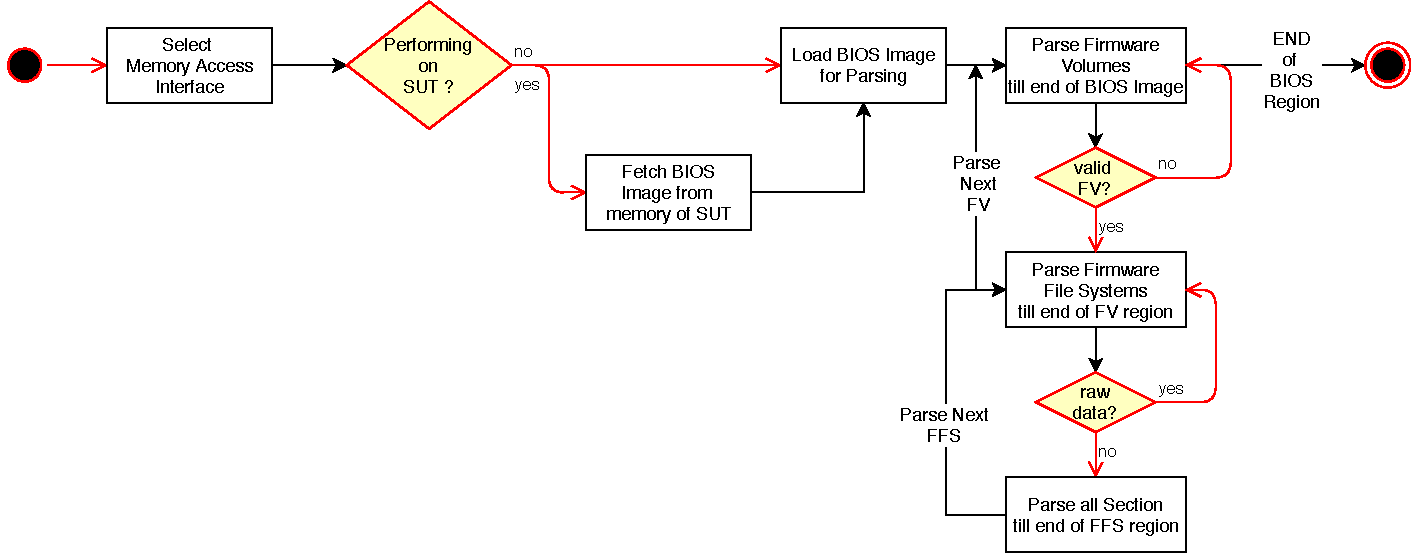
\includegraphics[width=\linewidth]{proposed-work/uefi-parser}
	\caption{Flow of Parser}\label{fig:uefi-parser}
\end{figure}

As on both the cases BIOS Image is available to act on, the module will start the parsing of the BIOS image as interpretation described in Figure \ref{fig:bios-as-filesystem}. It parses All the valid firmware volumes only till the end of BIOS image (skips the free space or firmware volumes with invalid signature and GUID). Decompression of file system under the firmware volume if any is handled by the module too, for the decompression of file system it uses the binary for decompression technique available to public i.e. lzma, tianocore, brotli etc.


\subsubsection{Outcome of Module}
\begin{itemize}
	\item Human Readable interpretation of BIOS image is provided.
	\item Possible to debug the BIOS via setup knobs comparison.
	\item Lookup of order of the module in BIOS image as readable file system is also possible.
	\item Verification of integration of module via GUID can be done.
	\item Extracting and storing file system or module of BIOS image by GUID
	\item Summarizing changes of two BIOS image
\end{itemize}



% ========================================================================
% MODULE 3
% ========================================================================
\subsection{Module: Runtime UEFI variable Creation}\label{module-runtime-uefi-variable-creation}
Each variable in BIOS has a scope for each variable where Runtime support is one of the attribute, to simply state the run time variable one can interpret it as the variable which will be available during and after the completion boot flow (while OS is running). Such a variable require special access mechanism, which is carried out by the System Management mode \gls{smm} described in Section \ref{section-smm}.

Earlier Challenges are described as below:
\begin{itemize}
	\item Providing and maintaining native driver support from BIOS for creation of UEFI variable
	\item Setting of Build environment for non-BIOS development team
\end{itemize}

Note: As all the variable created at runtime the scope of such variable are limited to the flashing of the BIOS. i.e. when BIOS is flashed/re-flashed or updated, those variable won't be available on the SUT.

\subsubsection{Additional Tech Stack Used}
Below are the listed technologies consumed in development of this module in addition to the already specified requirements in Section \ref{subsection-requirements}
\begin{itemize}
	\item Flask
	\item Ajax
	\item jQuery
	\item Javascript
	\item HTML/CSS
	\item XML
	\item JSON
\end{itemize}

\subsubsection{Flow of the module}
\begin{figure}[!htbp]
	\centering
	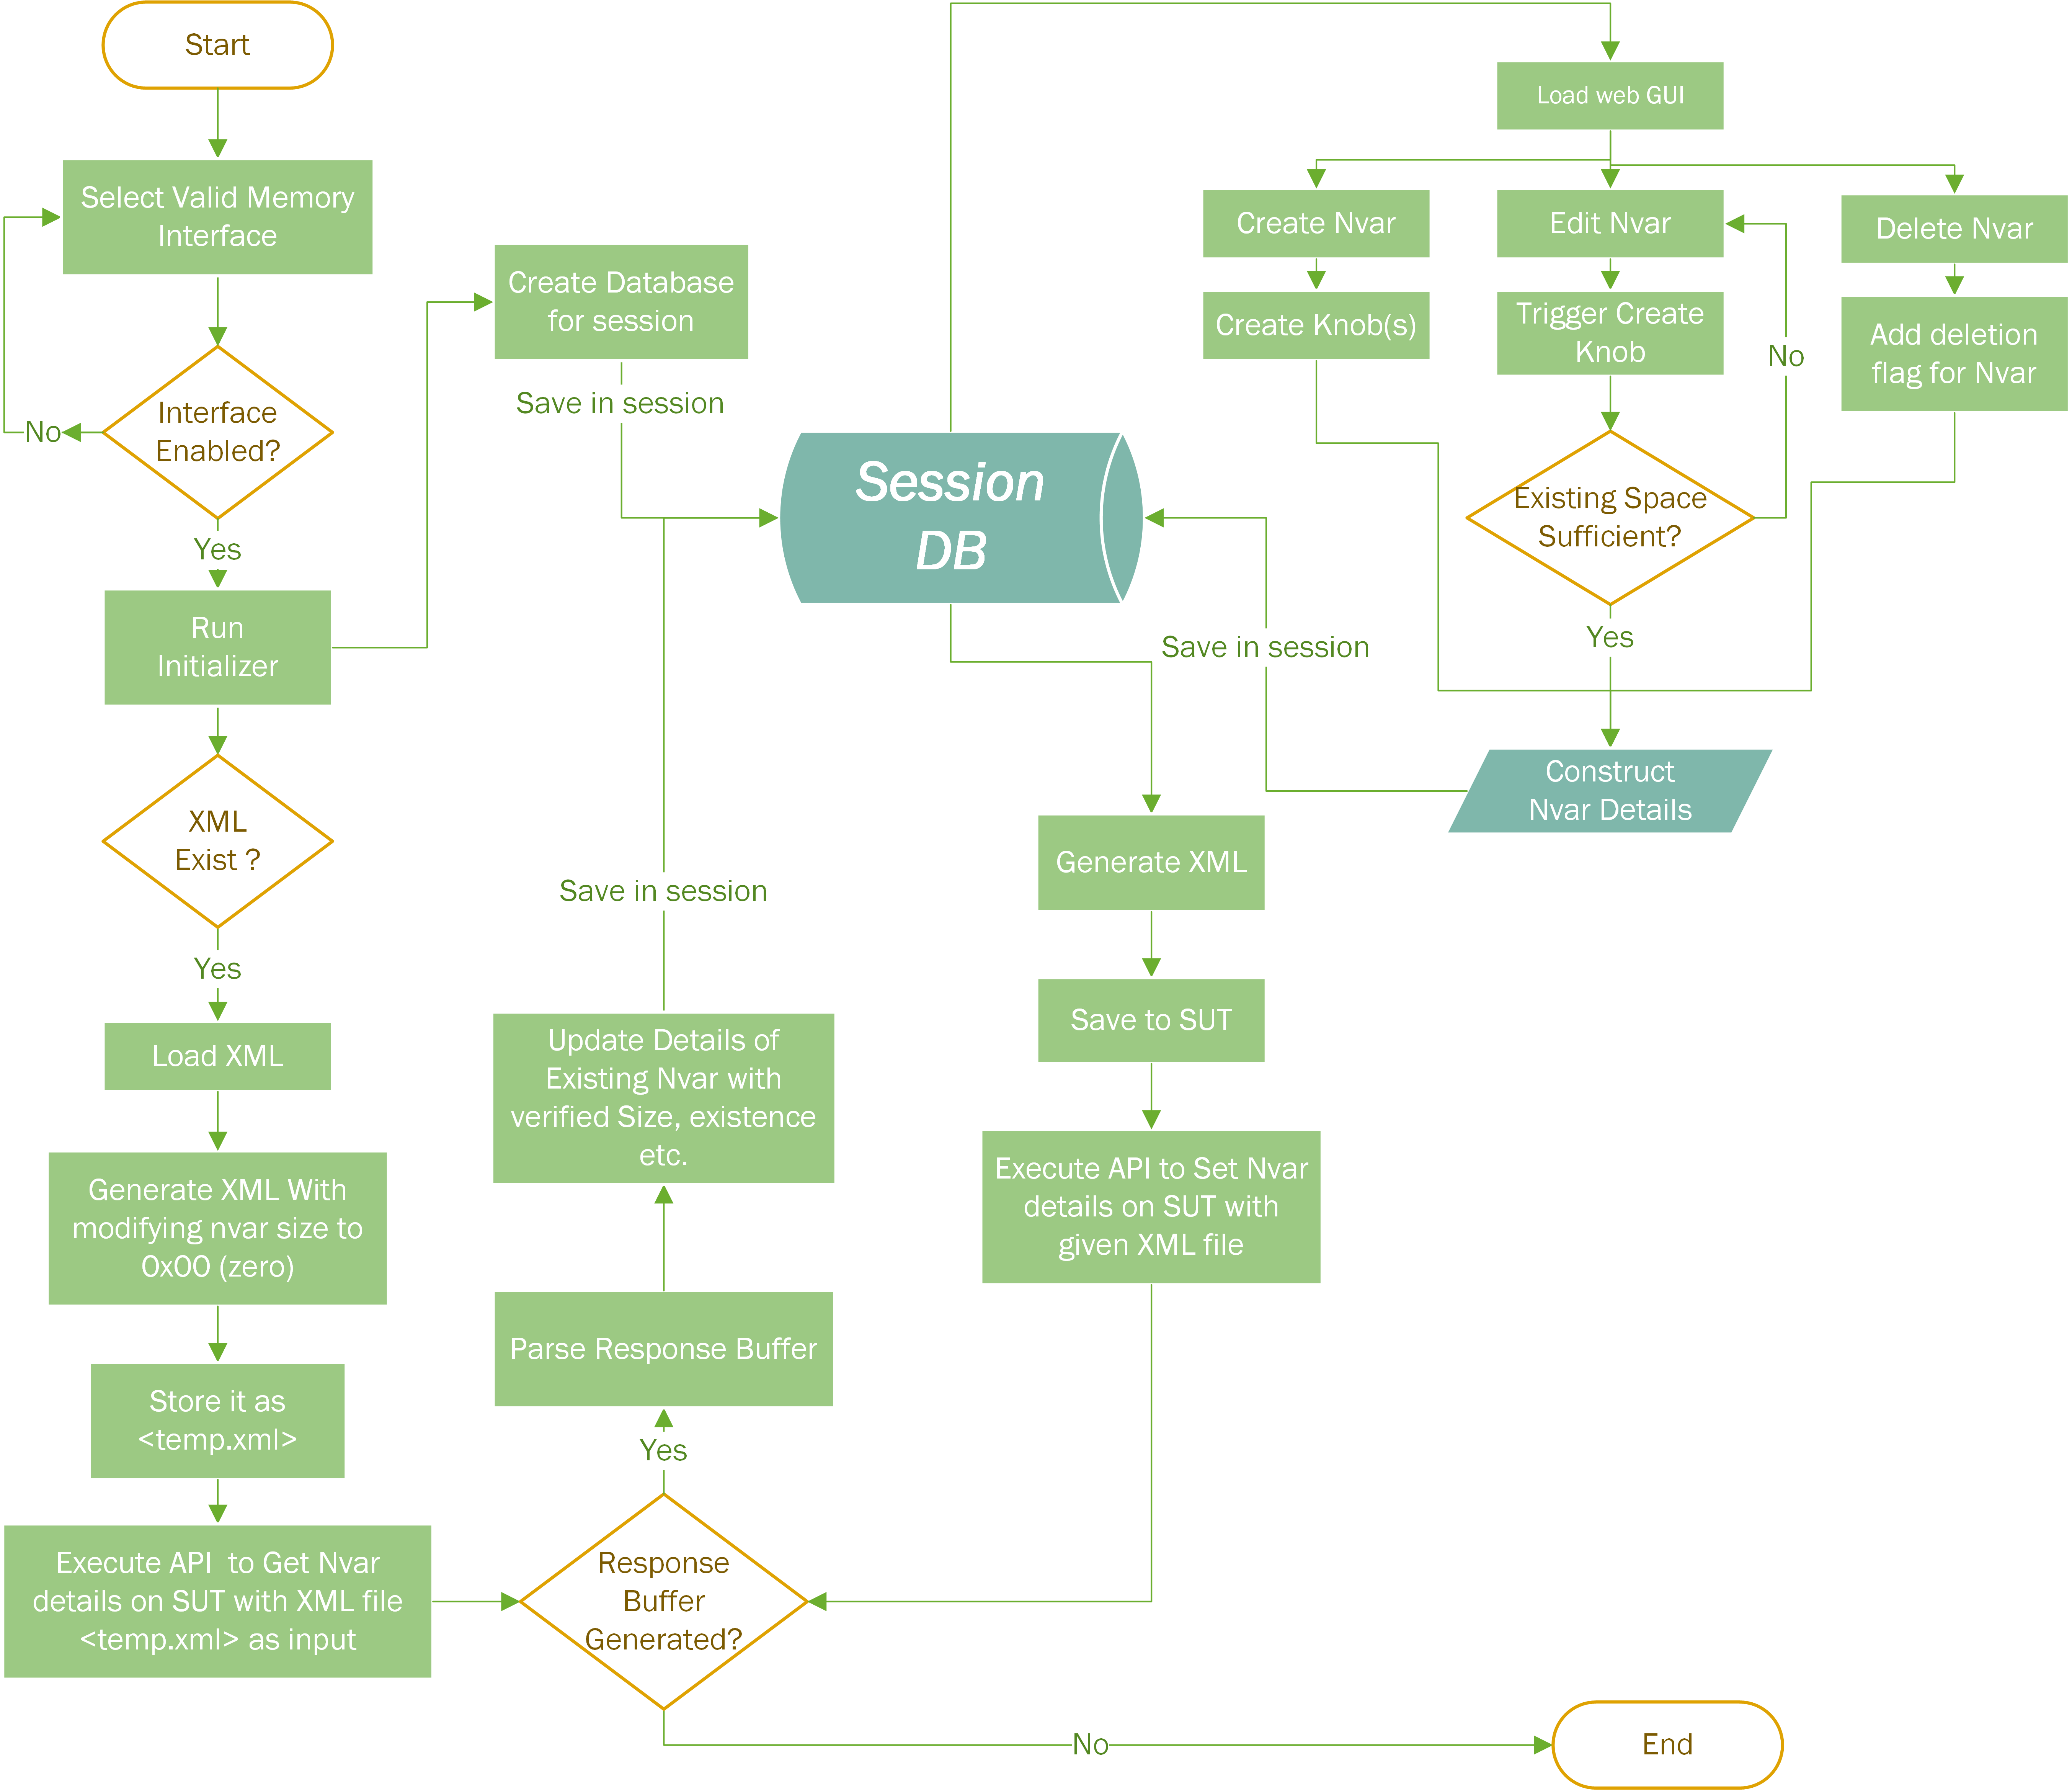
\includegraphics[width=1\linewidth]{proposed-work/nvar_web_GUI_flow}
	\caption{Flow of Nvar Web GUI}\label{fig:nvar_web_GUI_flow}
\end{figure}
The Flow of the module is described in section \ref{subsubsection-screenshots} along with screenshots which is easier to interpret the flow chart in Figure \ref{fig:nvar_web_GUI_flow}.

\subsubsection{Screenshots of Module}\label{subsubsection-screenshots}
Whenever the User launches the module the home page screen to select valid communication interface will appear as displayed in Figure \ref{fig:uefi-variable-home}. This is the crucial stage as if valid interface for communication is not selected one may not be able to use the functionality of the service.

\begin{figure}[!htbp]
	\centering
	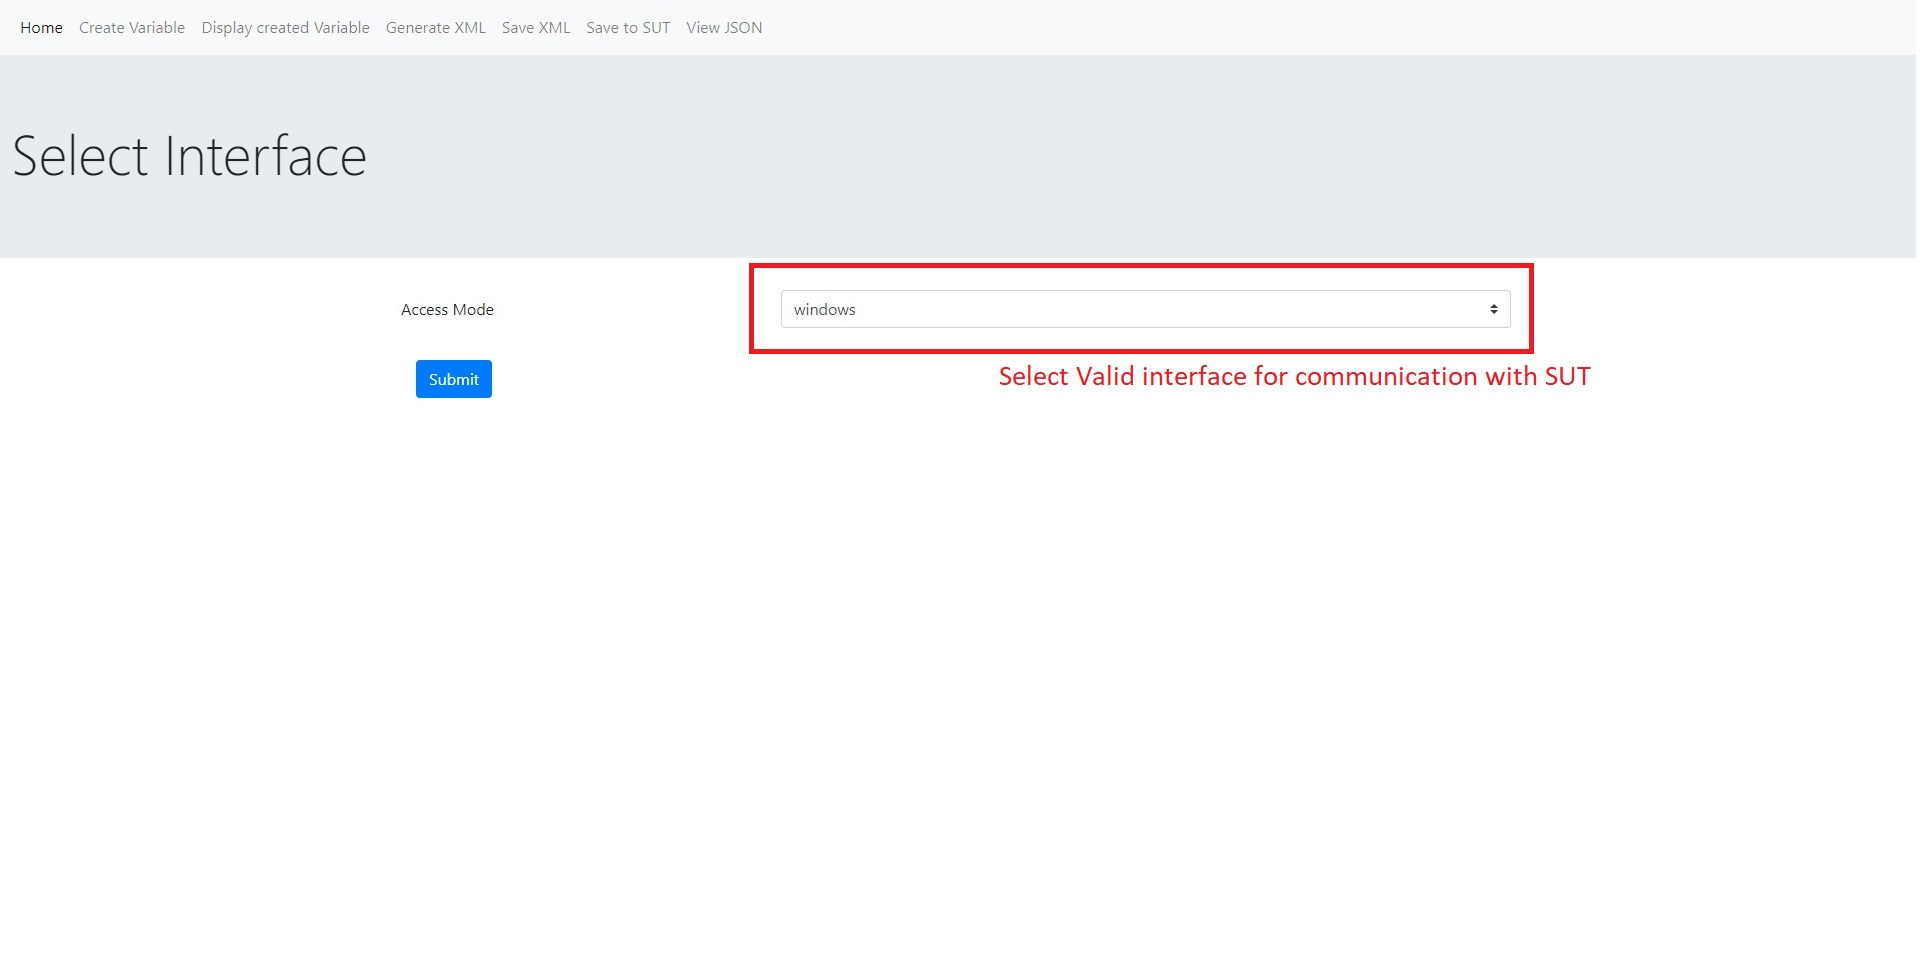
\includegraphics[width=\linewidth]{proposed-work/uefi-variables/home}
	\caption{Home Page to Create UEFI Variable}\label{fig:uefi-variable-home}
\end{figure}

After selection of valid Interface one may operate the desired options listed in navigation bar which are:

\begin{table}
	\centering
	\renewcommand{\arraystretch}{2}
	\caption{Navigation Bar Action}\label{table:navbar-action}
	\begin{tabular}{l | p {8cm}}
		Button & Interpretation
		\\ \hline \hline
		Create Variable & Opens a form to create new Variable as in Figure \ref{fig:uefi-variable-create-nvar}
		\\ \hline Display Created Variable & lists out created variable as in Figure \ref{fig:uefi-variable-created-option}
		\\ \hline Generate XML & Generate XML from the stored session database as in Figure \ref{fig:uefi-variable-generate-xml}
		\\ \hline Save XML & Saves the generated XML on the storage device
		\\ \hline Save to SUT & Applies the Pending changes action (Create/Delete/Modify) to the \gls{sut}
		\\ \hline View JSON & View the stored session database in the json format as in Figure \ref{fig:uefi-variable-represent-json}
		\\ \hline
	\end{tabular}
\end{table}


Figure \ref{fig:uefi-variable-created-option} lists the variable created under the current session which is to be applied 
\begin{figure}[!htbp]
	\centering
	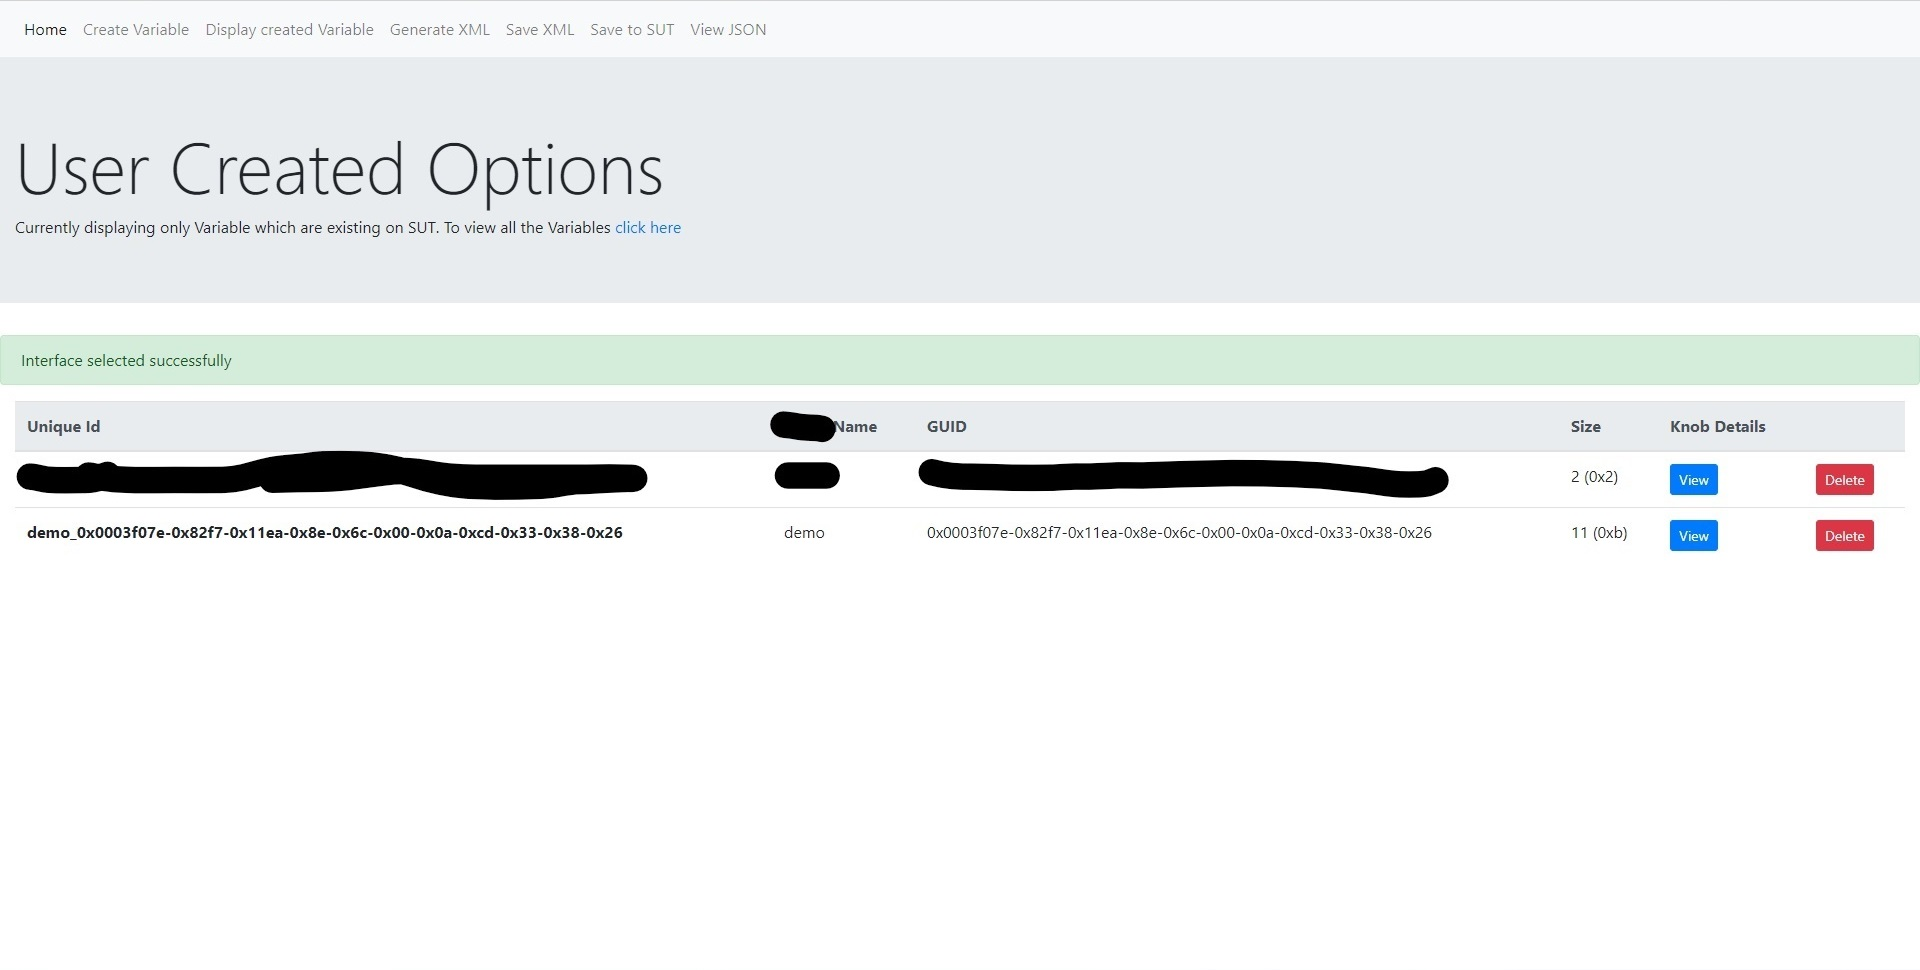
\includegraphics[width=\linewidth]{proposed-work/uefi-variables/created-option}
	\caption{Variables created or exists on \gls{sut}}\label{fig:uefi-variable-created-option}
\end{figure}

Figure \ref{fig:uefi-variable-create-nvar} displays form which allows user to create Variable, where user needs to specify the name of the variable with certain restriction of input field. To identify and lookup the Variable the GUID is required which is automatically generated by the module with required format, however if user wishes then they can modify the GUID.
\begin{figure}[!htbp]
	\centering
	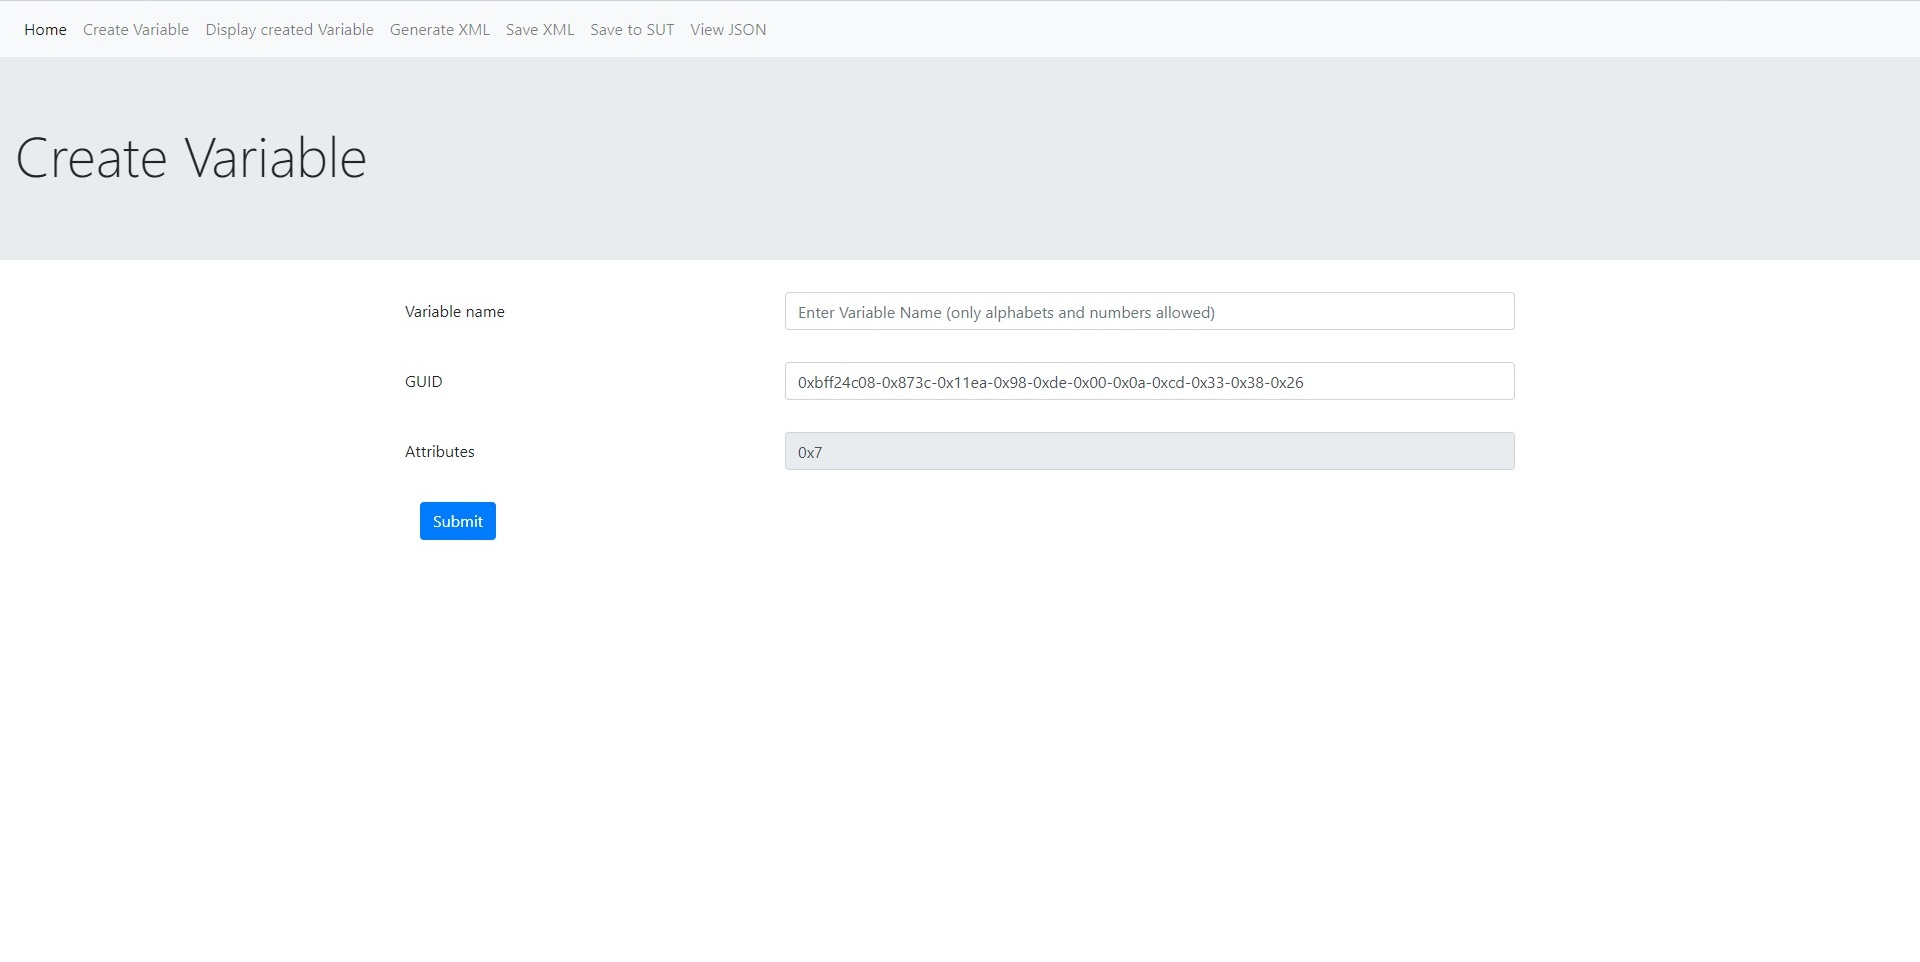
\includegraphics[width=\linewidth]{proposed-work/uefi-variables/create-nvar}
	\caption{Create new UEFI Variable on \gls{sut}}\label{fig:uefi-variable-create-nvar}
\end{figure}


Figure \ref{fig:uefi-variable-var-options} opens the list of the options if created and allows to edit their current values too. However one can also add the new option to the Variable. It allows user to create various types of options under the variable which are oneof type as in Figure \ref{fig:uefi-variable-add-option}, string type as in Figure \ref{fig:uefi-variable-string}, numeric type as in Figure \ref{fig:uefi-variable-numeric} and the checkbox type which allows user to toggle the option value in as Boolean interpretation. Common fields for creating options including its name, type, description and size.
\begin{figure}[!htbp]
	\centering
	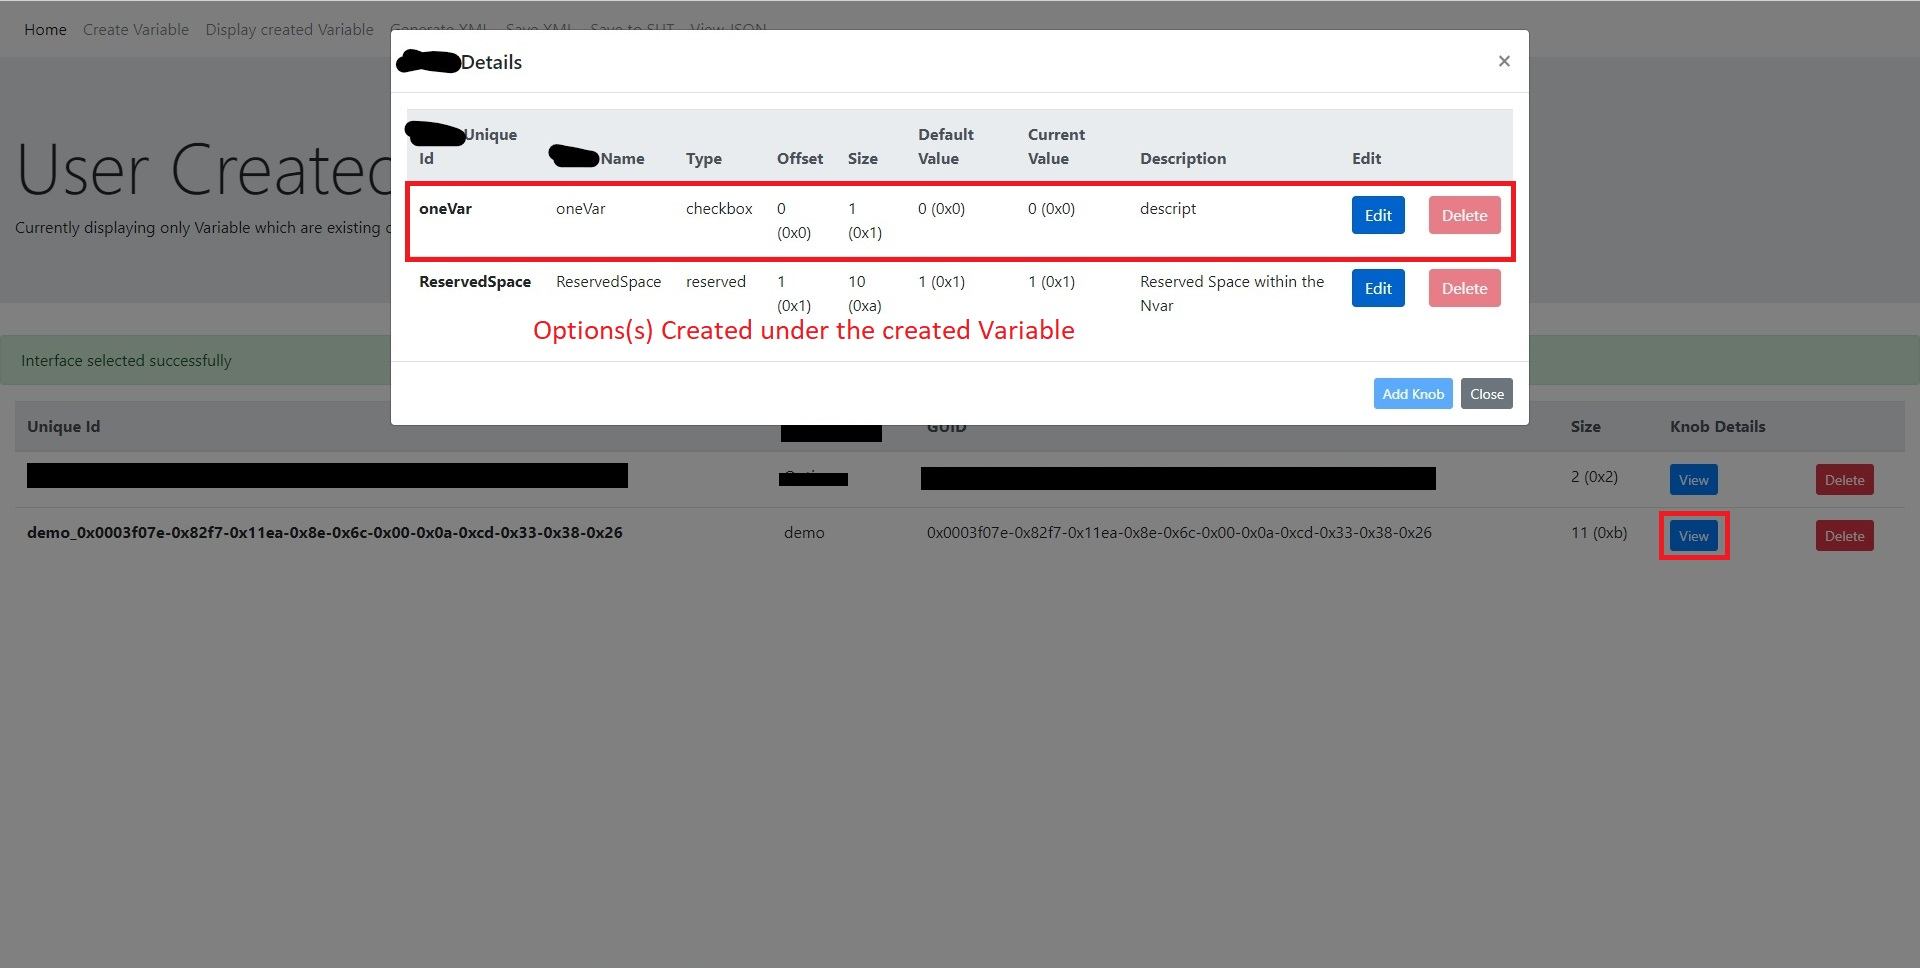
\includegraphics[width=\linewidth]{proposed-work/uefi-variables/var-options}
	\caption{Options listed under Variable}\label{fig:uefi-variable-var-options}
\end{figure}

If user wants to change the value set for the variable created while creation of option as described in Figure \ref{fig:uefi-variable-edit-option} forms one can actually modify the value.
\begin{figure}[!htbp]
	\centering
	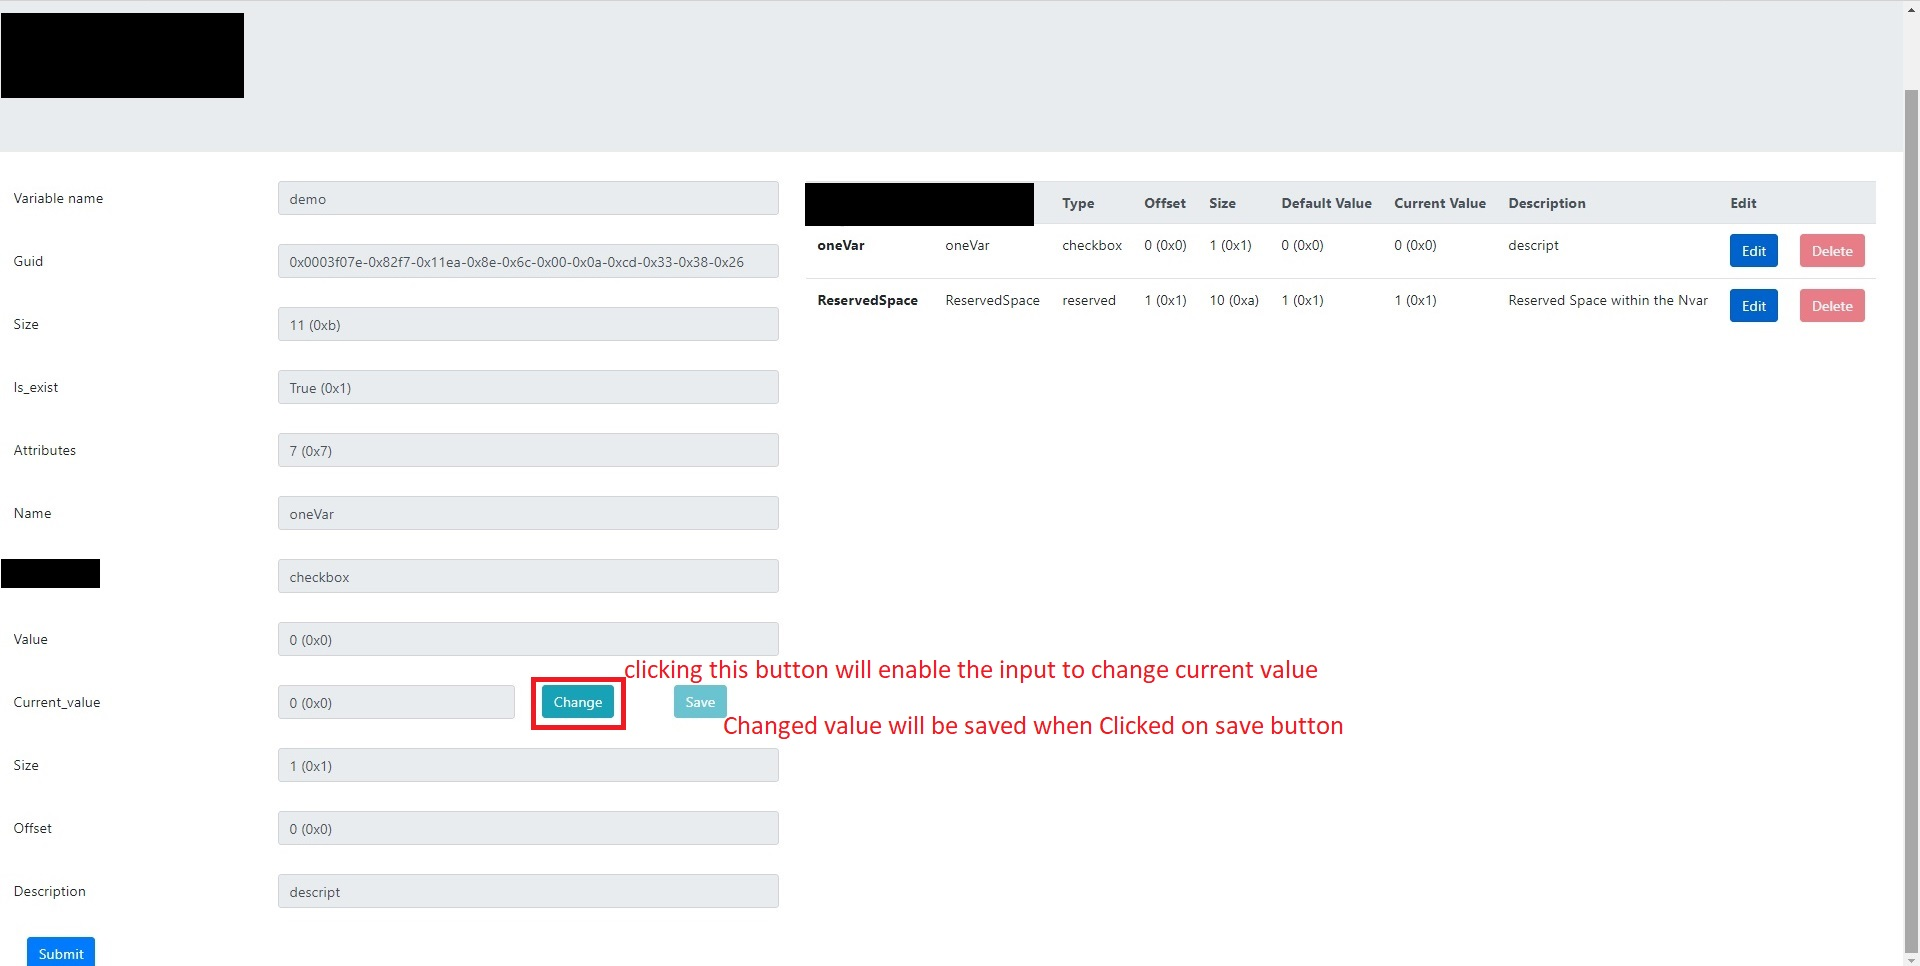
\includegraphics[width=\linewidth]{proposed-work/uefi-variables/edit-option}
	\caption{Edit the Existing Option Created under Variable \gls{sut}}\label{fig:uefi-variable-edit-option}
\end{figure}

The highlighted prompt in Figure \ref{fig:uefi-variable-add-option} allows user to create the choices for the option where one of the multiple values to be selected as a result, By clicking \verb|Add Option| button user can create choices and under drop down menu besides Value, user can select default value to be selected for the option. 
\begin{figure}[!htbp]
	\centering
	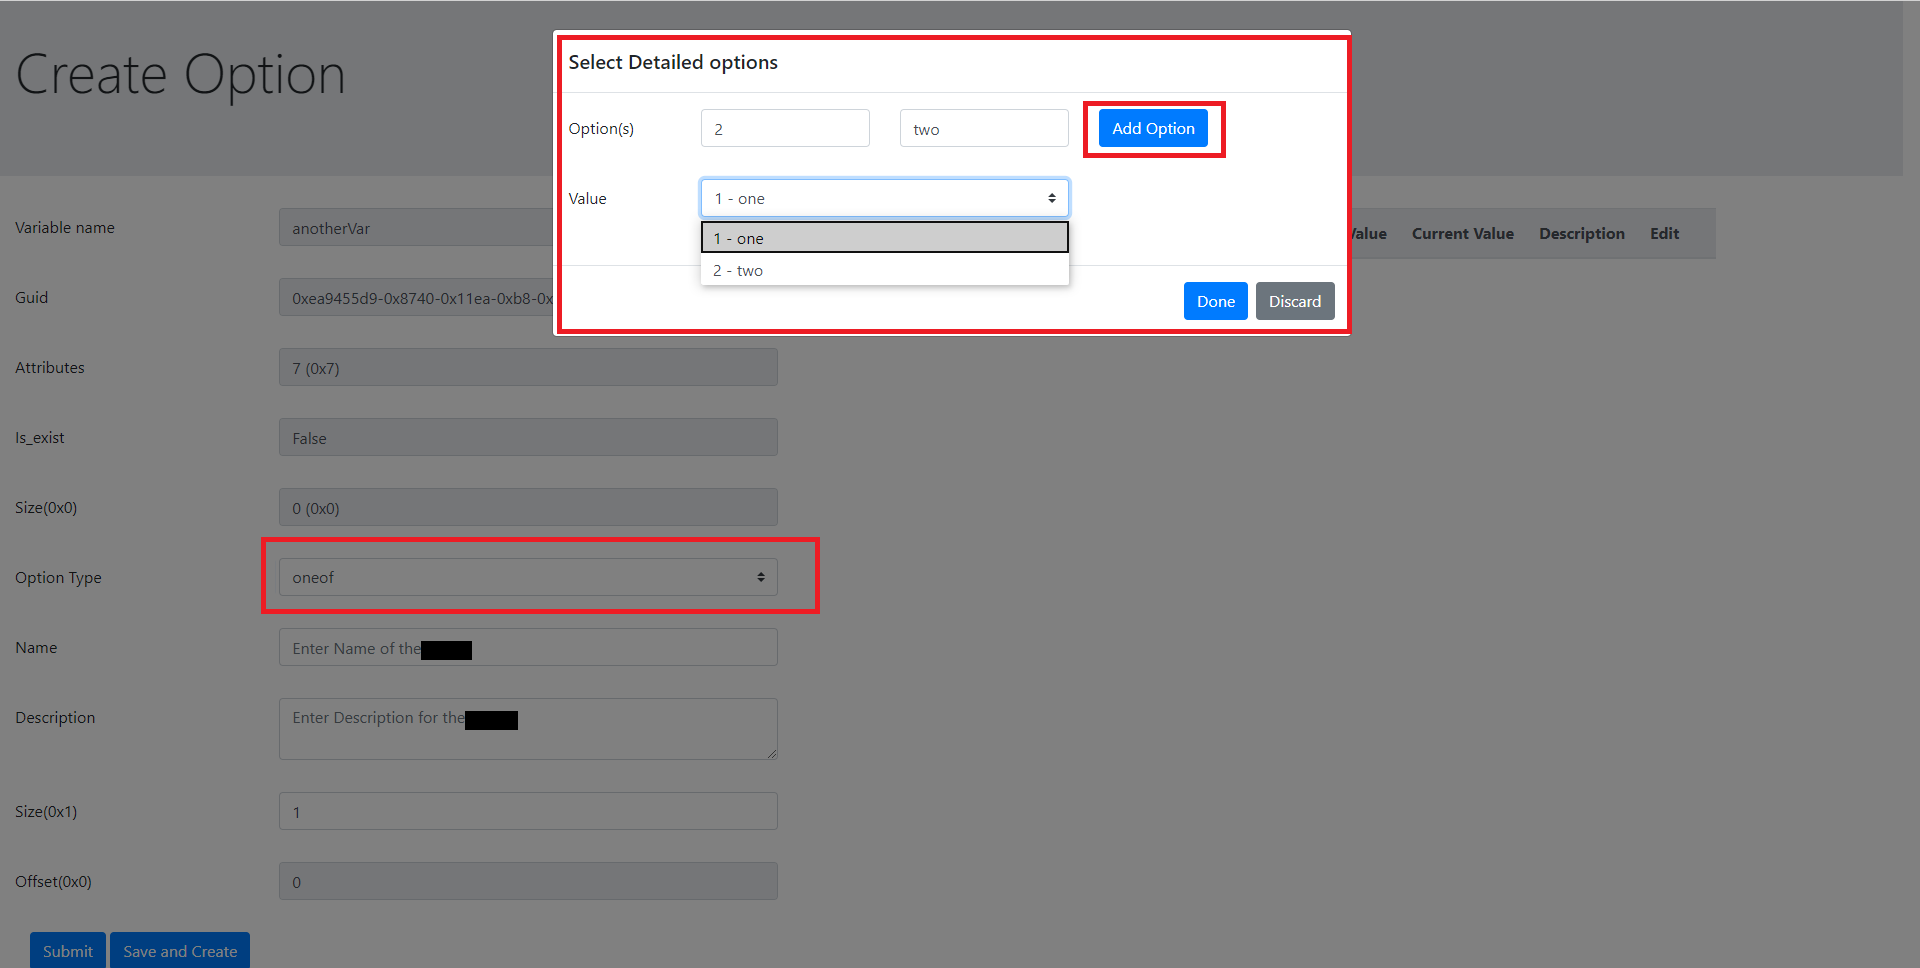
\includegraphics[width=\linewidth]{proposed-work/uefi-variables/add-option}
	\caption{Create New Option(s) under Variable - Oneof Type}\label{fig:uefi-variable-add-option}
\end{figure}

Option type string as in Figure \ref{fig:uefi-variable-string} allows user to create a option which accepts minimum and maximum characters to be supported in the string as well as the default string value to be selected. 
\begin{figure}[!htbp]
	\centering
	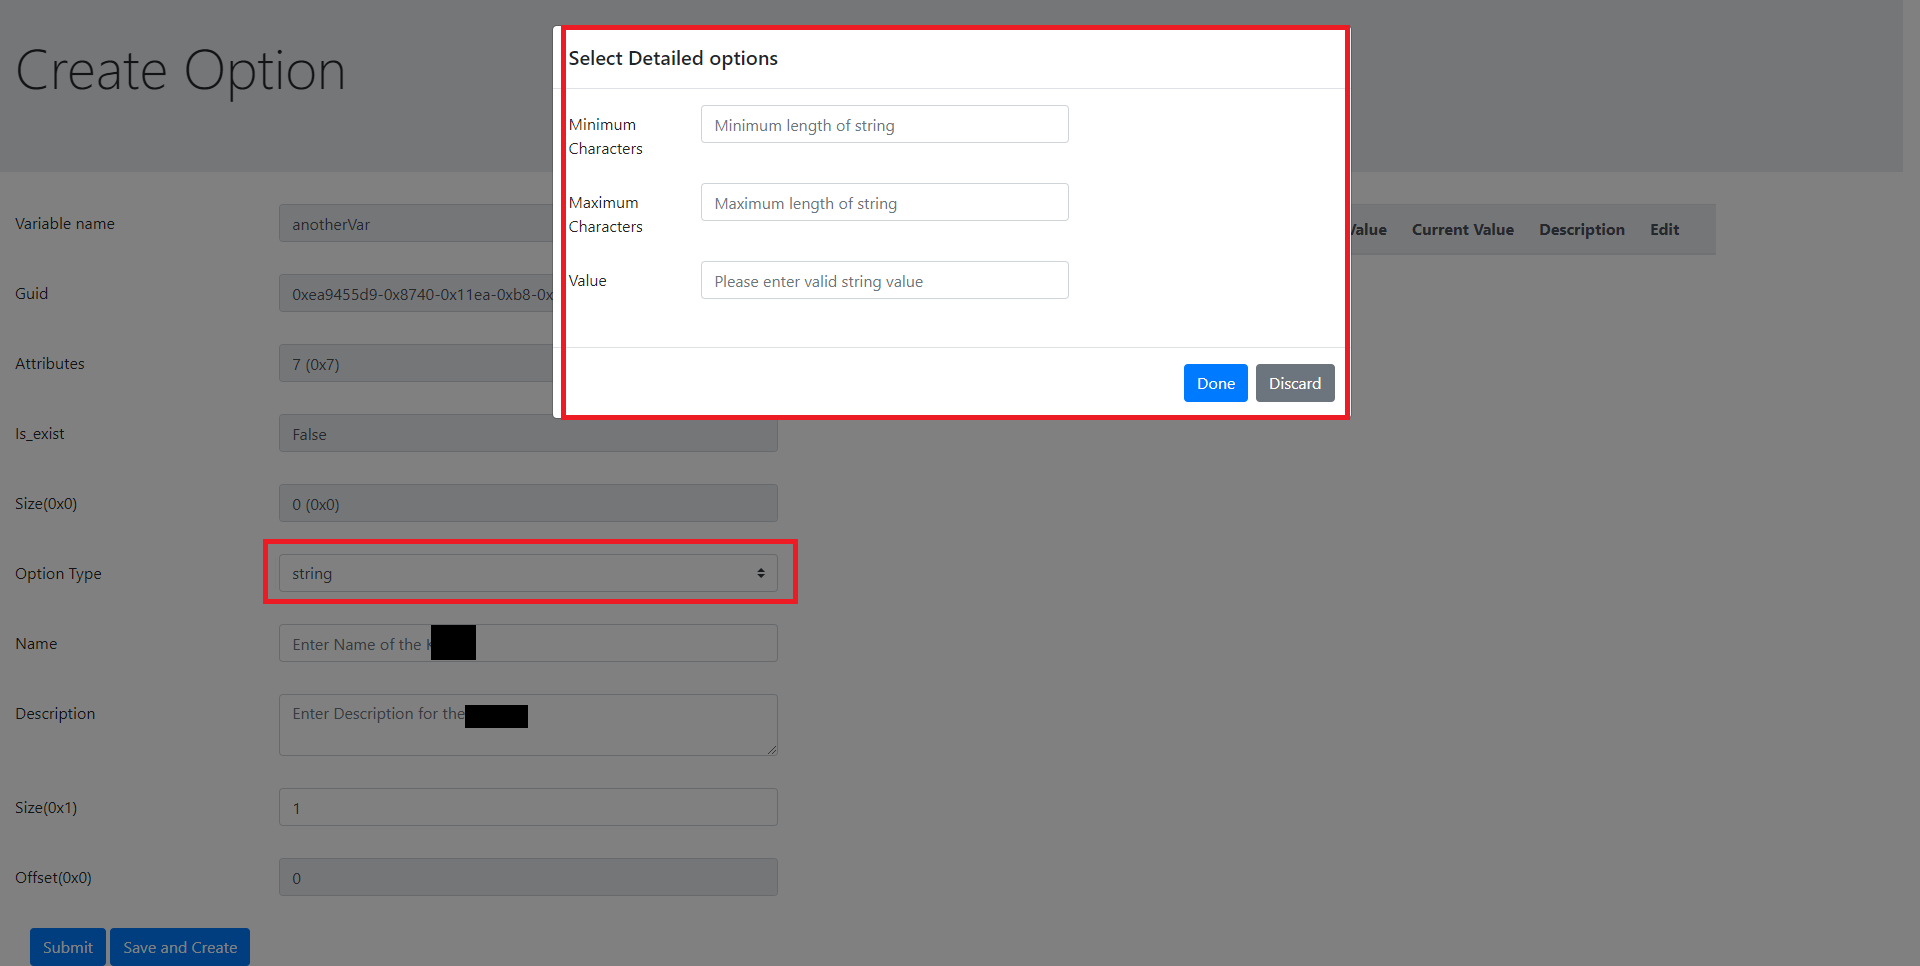
\includegraphics[width=\linewidth]{proposed-work/uefi-variables/string}
	\caption{Create New Option(s) under Variable - String Type}\label{fig:uefi-variable-string}
\end{figure}

To set the numeric input for the option, minimum and maximum value along with the default value to be set as in Figure \ref{fig:uefi-variable-numeric}
\begin{figure}[!htbp]
	\centering
	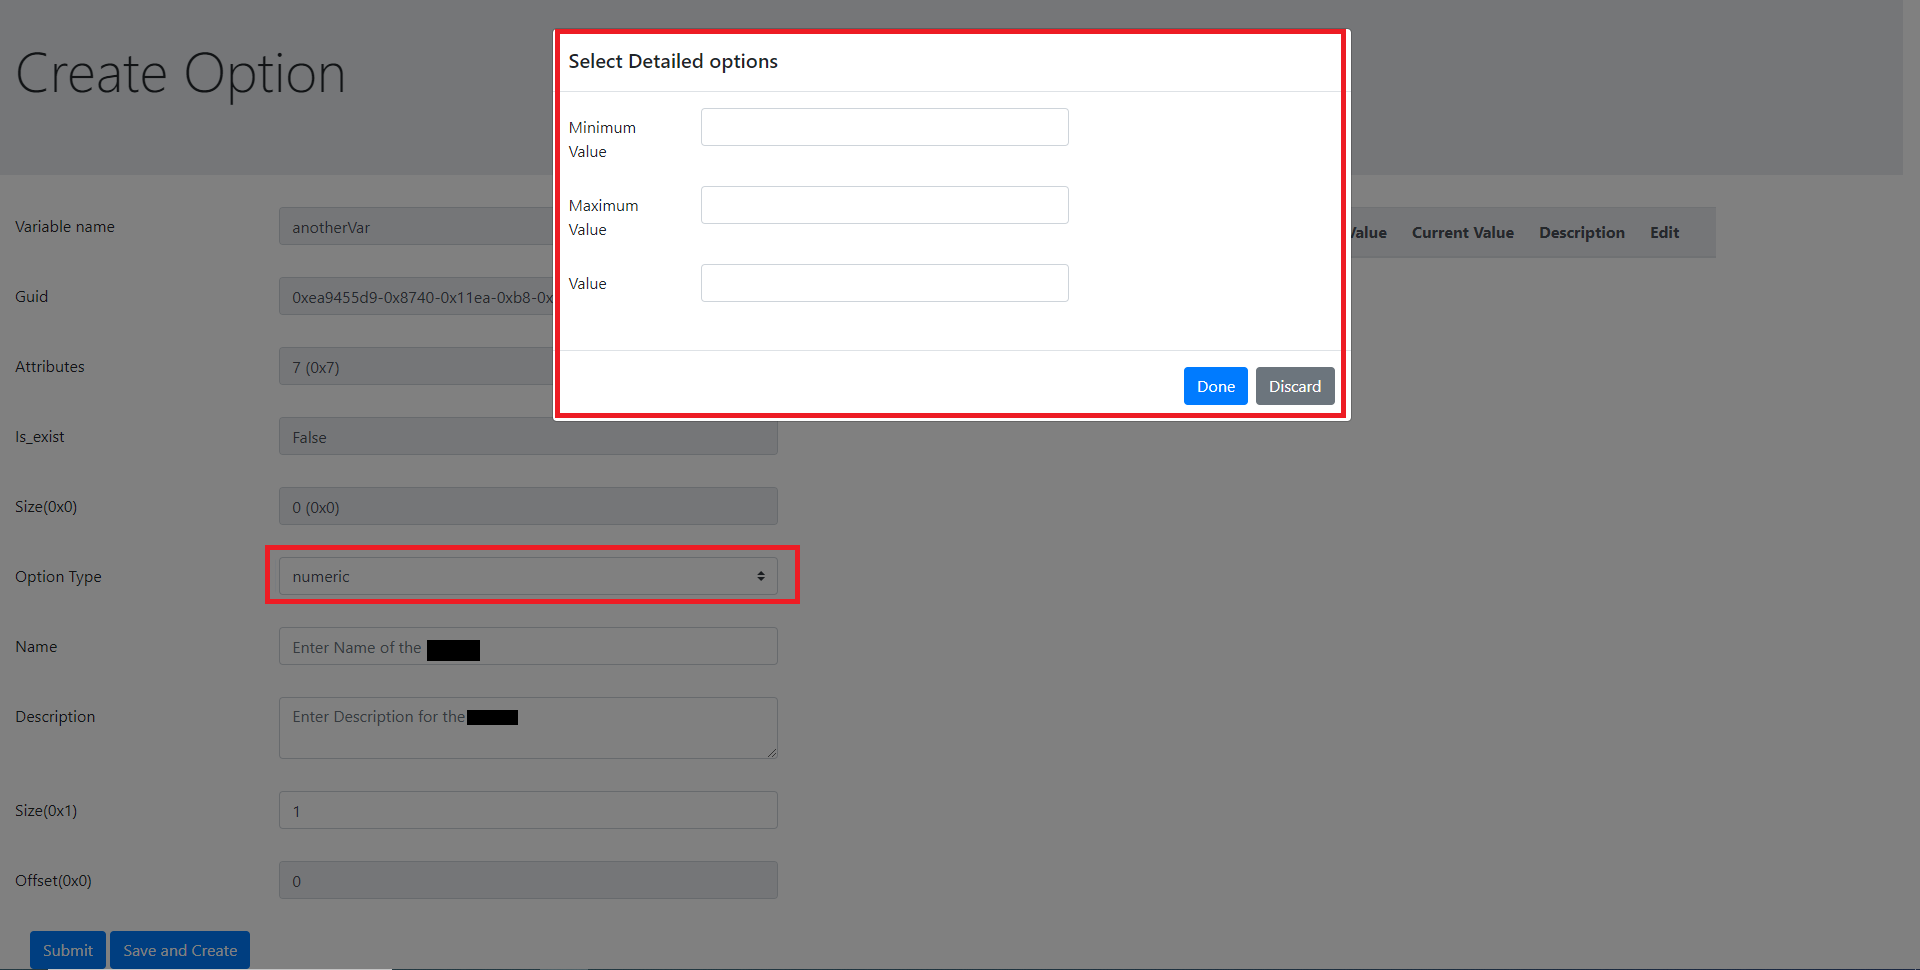
\includegraphics[width=\linewidth]{proposed-work/uefi-variables/numeric}
	\caption{Create New Option(s) under Variable - Numeric Type}\label{fig:uefi-variable-numeric}
\end{figure}

For the future use one can create a reserved space under the UEFI variable as in Figure \ref{fig:uefi-variable-reserved-space}
\begin{figure}[!htbp]
	\centering
	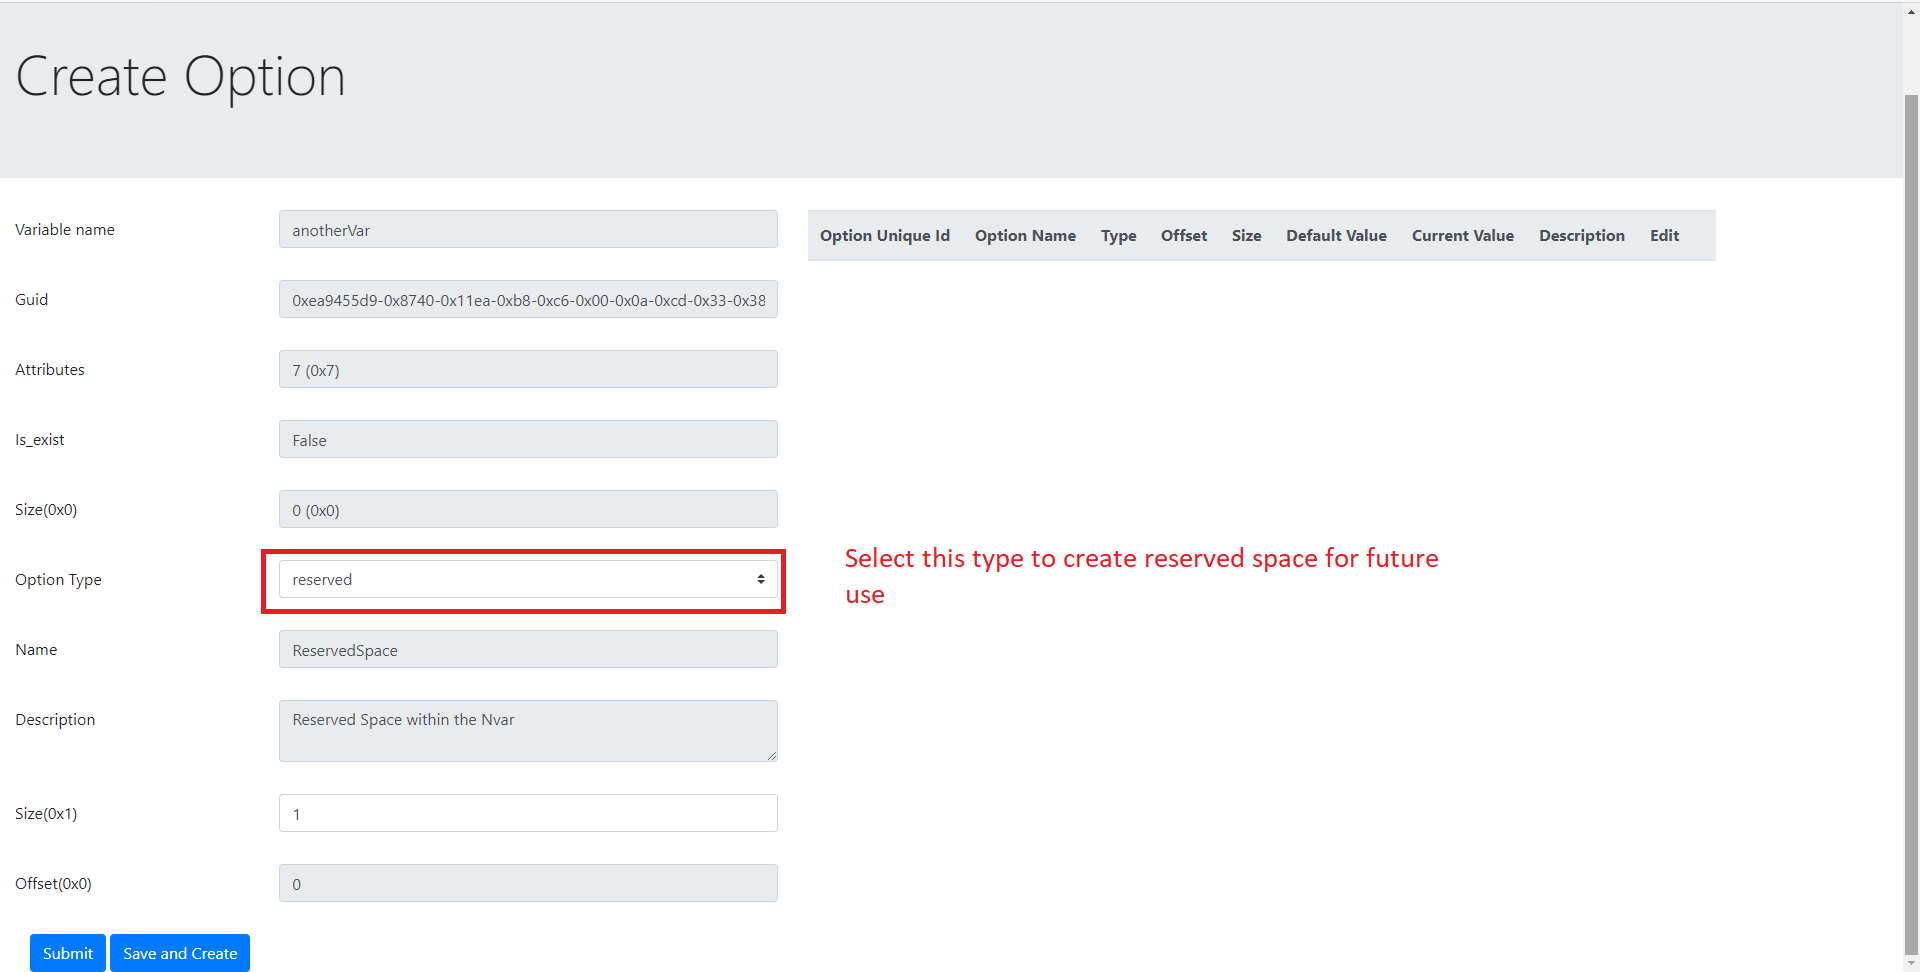
\includegraphics[width=\linewidth]{proposed-work/uefi-variables/reserved-space}
	\caption{Create Reserved Space for future use under Variable}\label{fig:uefi-variable-reserved-space}
\end{figure}


Figure \ref{fig:uefi-variable-generate-xml} shows the XML which is generated from the existing and newly created variables and options under it.
\begin{figure}[!htbp]
	\centering
	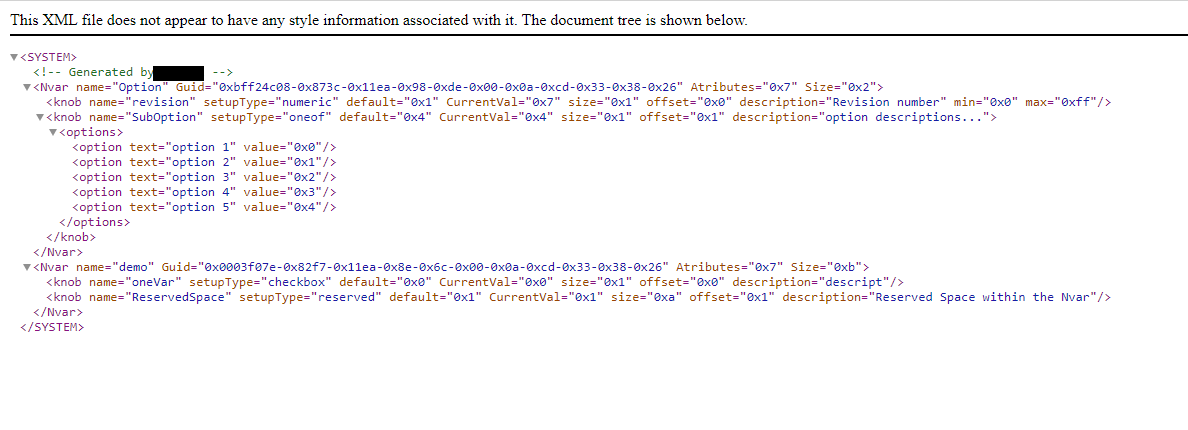
\includegraphics[width=\linewidth]{proposed-work/uefi-variables/generate-xml}
	\caption{Generate XML \gls{sut}}\label{fig:uefi-variable-generate-xml}
\end{figure}

Figure \ref{fig:uefi-variable-represent-json} represents session data of existing and newly created data (if any) as json
\begin{figure}[!htbp]
	\centering
	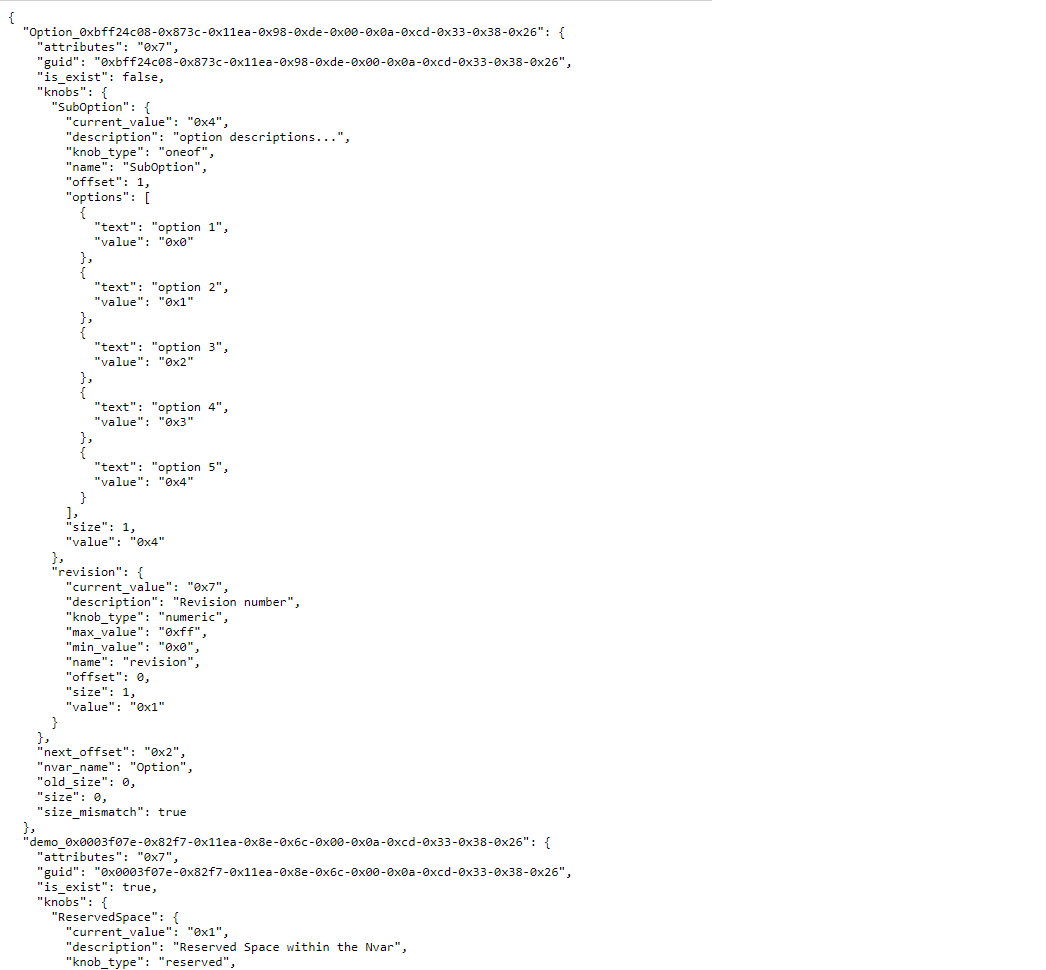
\includegraphics[width=\linewidth]{proposed-work/uefi-variables/represent-json}
	\caption{Generate XML \gls{sut}}\label{fig:uefi-variable-represent-json}
\end{figure}


\subsubsection{Outcome of the module}
\begin{itemize}
	\item Enables creation of UEFI variable from OS layer.
	\item Lifts headache of maintaining variable creation from BIOS development for individuals.
\end{itemize}


